\documentclass[a4paper,10pt]{report}

\usepackage{graphicx}
\usepackage{hyperref}
\usepackage{amsmath}
\usepackage{amssymb}
\usepackage{xspace}
\pagestyle{headings}
%\usepackage[margin=1.2in]{geometry}
\usepackage[left=2cm, right=2cm, top=2.5cm, bottom=2cm]{geometry}
\usepackage{float}
\restylefloat{table}
\usepackage{listings}
\usepackage{color}
\definecolor{gray}{rgb}{0.4,0.4,0.4}
\definecolor{darkblue}{rgb}{0.0,0.0,0.58}
\definecolor{attributeColor}{rgb}{0.96,0.517,0.29}
\definecolor{darkgreen}{rgb}{0,.392,0}
\definecolor{stringColor}{rgb}{0.6,0.2,0}
\usepackage{array,multirow}
\usepackage{longtable}
\usepackage{cleveref}
\usepackage{bbding}
\crefname{section}{�}{��}
\Crefname{section}{�}{��}
\usepackage[utf8]{inputenc}
\usepackage{tablefootnote}
\usepackage{algorithmic}

\newcommand{\myStartLine}{\par
  \kern8pt % space above the rules
  \hrule height 0.5pt
  \kern3pt % space below the rules
}
\newcommand{\myEndLine}{\par
  \kern3pt % space above the rules
  \hrule height 1.5pt
  \kern12pt % space below the rules
}

%\lstset{
%  basicstyle=\ttfamily,
%  columns=fullflexible,
%  showstringspaces=false,
%  commentstyle=\color{gray}\upshape
%  numbers=left,
%%  frame = single, 
%%  stepnumber=5
%}

\newcommand{\HRule}{\rule{\linewidth}{0.5mm}}

\lstdefinelanguage{XML}
{
  basicstyle=\ttfamily\footnotesize,
  morestring=[b]",
  morestring=[s]{>}{<},
  moredelim=[s][\bfseries\color{darkblue}]{<}{\ },
  moredelim=[s][\bfseries\color{darkblue}]{</}{>},
  moredelim=[l][\bfseries\color{darkblue}]{/>},
  moredelim=[l][\bfseries\color{darkblue}]{>},
  morecomment=[s]{<?}{?>},
  morecomment=[s]{<![CDATA[}{]]>},
  moredelim=[s][\bfseries\color{darkgreen}]{<!--}{-->},
  commentstyle=\color{darkgreen},
  stringstyle=\color{stringColor},
  identifierstyle=\color{red},
  keywordstyle=\color{attributeColor},
  morekeywords={oid,columnId,columnIdRef,symbId,symbolType,op,columnNum,columnType,
  valueType,inputTarget,blkId,blkIdRef,symbIdRef,xmlns,version,type,VariableMapping,
  IndividualMapping,schemaLocation,xs,xsi,NONMEMdataSet,matrixType,opType,order,
  math,ct,ds,mdef,mstep,mml,un,name,definition,writtenVersion,id,inputType,oidRef,catId,
  length,default,vectorIndex,diagDefault,offDiagDefault,row,column,numbRows,numbCols,
  dataSymbol,modelSymbol,ordered,compartmentNo,compNo,ordered,linkFunction,varId,
  censoringType,dataSymbol,modelSymbol,MarkovOrder,deviationMatrixType,implementedBy,
  argument,admNumber,transformId,transformIdRef} % list your attributes here
}

\lstdefinelanguage{MLXTRANcode} 
{
  basicstyle=\ttfamily\footnotesize,
  morestring=[b]",
  morestring=[s]{>}{<},
  moredelim=[s][\bfseries\color{darkblue}]{<}{\ },
  moredelim=[s][\bfseries\color{darkblue}]{</}{>},
  moredelim=[l][\bfseries\color{darkblue}]{/>},
  moredelim=[l][\bfseries\color{darkblue}]{>},
  morecomment=[s]{<?}{?>},
  morecomment=[s]{<!--}{-->},
  morecomment=[s]{<![CDATA[}{]]>},
  commentstyle=\color{darkgreen},
  stringstyle=\color{stringColor},
  identifierstyle=\color{black},
  keywordstyle=\color{attributeColor},
  morekeywords={dads} % list your attributes here
}

\lstdefinelanguage{NONMEMdataSet}
{
  basicstyle=\ttfamily\footnotesize,
  morestring=[b]",
  morestring=[s]{>}{<},
  moredelim=[s][\bfseries\color{darkblue}]{<}{\ },
  moredelim=[s][\bfseries\color{darkblue}]{</}{>},
  moredelim=[l][\bfseries\color{darkblue}]{/>},
  moredelim=[l][\bfseries\color{darkblue}]{>},
  morecomment=[s]{<?}{?>},
  morecomment=[s]{<!--}{-->},
  morecomment=[s]{<![CDATA[}{]]>},
  commentstyle=\color{darkgreen},
  stringstyle=\color{stringColor},
  identifierstyle=\color{black},
  keywordstyle=\color{attributeColor},
  morekeywords={kjkj} % list your attributes here
}


\newcommand{\cellml}{CellML\xspace}
\newcommand{\sbml}{SBML\xspace}
\newcommand{\sedml}{SED-ML\xspace}
\newcommand{\mathml}{MathML\xspace}
\newcommand{\uncertml}{UncertML\xspace}
\newcommand{\pml}{PharmML\xspace}
\newcommand{\pharmml}{PharmML\xspace}
\newcommand{\xelem}[1]{\texttt{<#1>}\index{XML Element!\texttt{<#1>}}}
\newcommand{\xatt}[1]{\texttt{#1}\index{XML Attribute!\texttt{#1}}}

\begin{document}

\begin{titlepage}
\begin{center}

% Upper part of the page. The '~' is needed because \\
% only works if a paragraph has started.

\includegraphics[width=0.35\textwidth]{./logo/ddmore_logo}~\\[1cm]

%\textsc{\LARGE }\\[1.5cm]
%
\textsc{\Large Internal Release}\\[0.5cm]

% Title
\HRule \\[0.4cm]
{ \huge \bfseries Extensions in PharmML 0.6.1 \\[0.4cm] }

\HRule \\[1.5cm]

% Author and supervisor
\begin{minipage}{0.5\textwidth}
\begin{flushleft} \large
\emph{Authors:}\\
Maciek J \textsc{Swat}\\
Sarala \textsc{Wimalaratne}\\
Niels Rode \textsc{Kristensen}
\end{flushleft}
\end{minipage}
%\begin{minipage}{0.4\textwidth}
%\begin{flushright} \large
%%\emph{with contributions from:} \\
%%Roberto \textsc{Bizzotto} \\
%%Marc \textsc{Lavielle}
%\end{flushright}
%\end{minipage}



\vfill

% Bottom of the page
{\large \today \\}
% {Version 0.4 was released on July 16, 2014}

\end{center}
\end{titlepage} 
	
%\maketitle

\tableofcontents


%%%%%%%%%%%%%%%%%%%%%%%%%%%%%%%%%%%%%%%%%%%%%%%%%%%%%%%%%%%%%%%%%%%%%%
%%%%%%%%%%%%%%%%%%%%%%%%%%%%%%%%%%%%%%%%%%%%%%%%%%%%%%%%%%%%%%%%%%%%%%%
%%%%%%%%%%%%%%%%%%%%%%%%%%%%%%%%%%%%%%%%%%%%%%%%%%%%%%%%%%%%%%%%%%%%%%%
%%%%%%%%%%%%%%%%%%%%%%%%%%%%%%%%%%%%%%%%%%%%%%%%%%%%%%%%%%%%%%%%%%%%%%%
\chapter{Overview}

This document describes extensions and changes in \pml compared to the
previously released version 0.3.1. It is not intended to serve as a proper specification. 
The next public release, due in M42, will come with a fully updated specification document.
The current document introduces the discrete data models, delay differential equations,
extended vector and matrix support and a few new language elements and other corrections/changes.
The appendix \ref{chapter:codeExamples} contains examples of implemented discrete 
data models.

\section{Major changes/extensions in version 0.4}
The following table summarises the changes described in detail in Chapters \ref{chapter:DDmodels} and 
\ref{chapter:other04extensions}.

\begin{center}
\begin{longtable}{lll}
\hline
\hline
\pml element 			&  version $\le$ 0.3.1 			& version 0.4 \\
or modelling aspect 		&							& \\
\hline
Discrete data models 	& \emph{not supported}			& \xelem{Discrete} with child elements such as {\color{red} \scshape{new}} \\
\hline
Extended matrix definition & basic support 		 		& \xelem{Matrix} with a number of child elements such as\\
 (see \textsection\ref{subsec:matrixStructure})	& 			& \xelem{MatrixRow}, \xelem{MatrixCell}, \\
					& 							& \xelem{MatrixBlock} and attributes \xatt{matrixType}, \\
					&							& \xatt{diagDefault}, \xatt{offDiagDefault} and others  \\ 
\hline
\caption{Overview of major differences between versions 0.4 and 0.3.1}
\label{figTable:overviewTable}
\end{longtable}
\end{center}



%%%%%%%%%%%%%%%%%%%%%%%%%%%%%%%%%%%%%%%%%%%%%%%%%%%%%%%%%%%%%%%%%%%%%%
\section{Vectors and Matrices -- reloaded}
\label{sec:vectorsAndMatrices}
 \pml has been equipped with vector support and version 0.3.1 introduced additionally 
 the concept of a matrix for the purpose of encoding correlation/covariance matrices. 
Unfortunately, both structures turned out to be insufficient. The vectors were not ready 
to accept other than numerical entries and both vectors and matrices could not be
indexed. Version 0.4 solves these issues. The schema for these two elements is based
on two standards, one dealing with mathematical notation, MathML \cite{mathml3:2010}, 
and another one with data mining models, PMML \cite{pmml:2014}, and comes with 
a wide range of features enabling flexible handling of vectors and matrices via a 
flexible indexing schema.

\begin{figure}[htbp]
\centering
 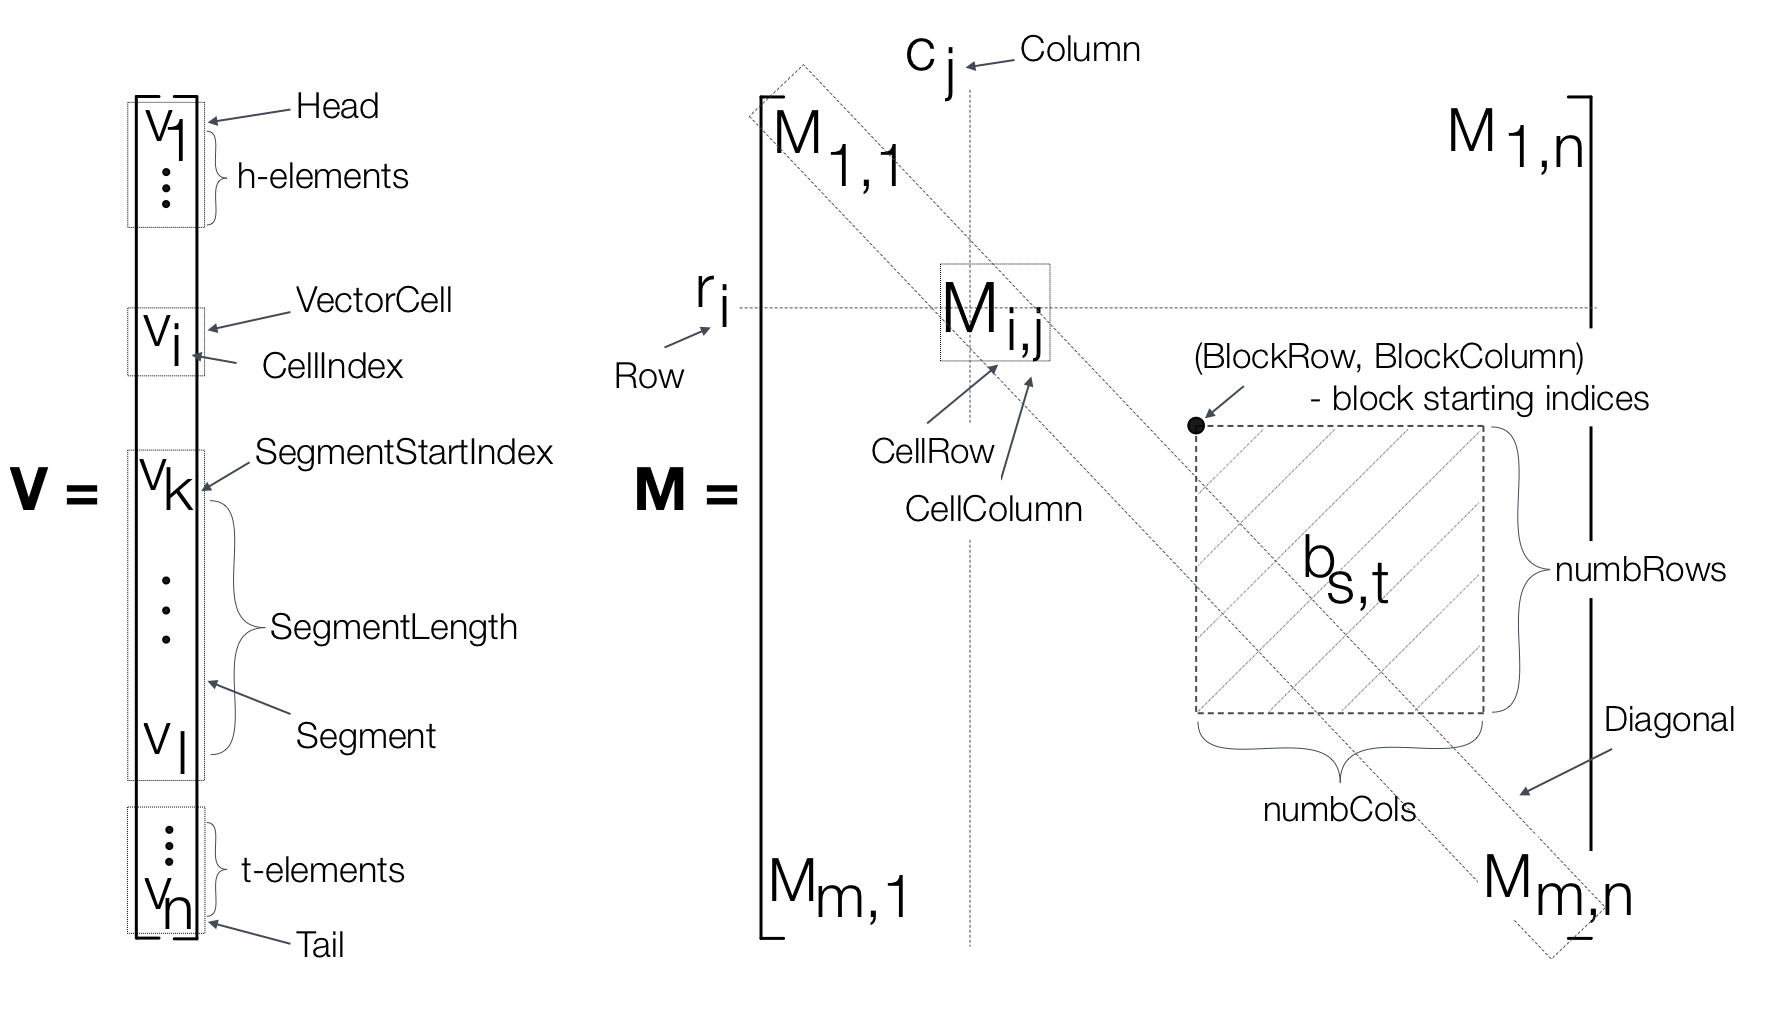
\includegraphics[width=160mm]{pics/VectorMatrixOverview.jpg}
\caption{Vector and matrix -- vocabulary and structure overview.}
\label{fig:vectorMatrix}
\end{figure}



%%%%%%%%%%%%%%%%%%%%%%%%%%%%%%%%%%%%%%%%%%%%%%%%%%%%%%%%%%%%%%%%%%%%%%
\subsection{Vector structure with examples {\color{red} \scshape{*}}}
\label{subsec:vectorType}
Vectors are defined to be column vectors. Row vectors can be created by taking
the transpose (with the \emph{transpose} operation still to be defined) of a column vector. 

\subsubsection{Populating vectors}
\begin{itemize}
\item
Elements
\begin{itemize}
\item
\xelem{VectorElements} is used to define all vector elements without indexing and takes any 
combination of the following items
\begin{itemize}
\item
\xelem{Scalar} and/or \xelem{SymbRef}
\item
\xelem{Equation} -- vector elements can contain expressions  {\color{red} \scshape{NEW}}
\item
\xelem{Sequence}
\end{itemize}
\item
\xelem{VectorCell} is used to define single elements of the vector by specifying
\begin{itemize}
\item
\xelem{CellIndex} {\color{red} \scshape{renamed}} 
\item
\xelem{Scalar}, \xelem{SymbRef} or
\item
\xelem{Equation} -- vector cells can also contain expressions {\color{red} \scshape{NEW}}
\end{itemize}
\item
\xelem{VectorSegment} allows to encode $n$ consecutive elements using the 
\begin{itemize}
\item
\xelem{SegmentStartIndex} {\color{red} \scshape{renamed}} -- marks the start index within a vector
\item
\xelem{SegmentLength} --  the length of the segment and
\item
\xelem{VectorElements} as explained above.
\end{itemize}
\item
all indexes can contain expressions  {\color{red} \scshape{NEW}}
\end{itemize}
\item
Attributes
\begin{itemize}
\item
\xatt{default} stands for the value of not explicitly specified elements -- necessary when 
sparse vectors are encoded using \xelem{VectorCell} or \xelem{VectorSegment}
\item
\xatt{length} of the vector -- required in certain situations, see \xatt{default} comments above.
\end{itemize}
\end{itemize}
Table \ref{tab:vectorsComparison} show two examples how you can encode vectors.

\begin{table}[ht!]
\setlength{\tabcolsep}{10pt}
\begin{center}
\begin{tabular}{ll}
  \hline
  \hline
 \pml version $\le$ 0.3.1 &  \pml version 0.4 \\
  \hline
% \multicolumn{2}{c}{encoding [0,2,0,0,5,0,0,0,0,0]}  \\
%  \hline
  \lstset{language=XML}
\begin{lstlisting}
<ct:Vector>
    <ct:Real>0</ct:Real>
    <ct:Real>2</ct:Real>
    <ct:Real>0</ct:Real>
    <ct:Real>0</ct:Real>
    <ct:SymbRef symbIdRef="fifthElement"/>
    <ct:Real>0</ct:Real>
    <ct:Real>0</ct:Real>
    <ct:Real>0</ct:Real>
    <ct:Real>0</ct:Real>
    <ct:Real>0</ct:Real>
</ct:Vector>
\end{lstlisting}
&
\lstset{language=XML}
\begin{lstlisting}
<ct:Vector length="10">
    <ct:VectorElements>
        <ct:Real>0</ct:Real>
        <ct:Real>2</ct:Real>
        <ct:Real>0</ct:Real>
        <ct:Real>0</ct:Real>
        <ct:SymbRef symbIdRef="fifthElement"/>
        <ct:Real>0</ct:Real>
        <ct:Real>0</ct:Real>
        <ct:Real>0</ct:Real>
        <ct:Real>0</ct:Real>
        <ct:Real>0</ct:Real>
    </ct:VectorElements>
</ct:Vector>
\end{lstlisting}  
\\
& OR
\\
--
&
\lstset{language=XML}
\begin{lstlisting}
<ct:Vector default="0" length="10">
    <ct:VectorCell>
        <ct:VectorIndex>
            <ct:Int>2</ct:Int>
        </ct:VectorIndex>
        <ct:Real>2</ct:Real>
    </ct:VectorCell>
    <ct:VectorCell>
        <ct:VectorIndex>
            <ct:Int>5</ct:Int>
        </ct:VectorIndex>
        <ct:SymbRef symbIdRef="fifthElement"/>
    </ct:VectorCell>
</ct:Vector>
\end{lstlisting} 
\\
%\hline
% \multicolumn{2}{c}{encoding [1,1,3,4,5,6,1,1,1,1]}  \\
%\hline
%-- & \lstset{language=XML}
%\begin{lstlisting}
%<ct:Vector default="1" length="10">
%    <ct:VectorSegment>
%        <ct:StartIndex>3</ct:StartIndex>
%        <ct:EndIndex>6</ct:EndIndex>
%    </ct:VectorSegment>
%</ct:Vector>
%\end{lstlisting} \\
  \hline
  \end{tabular}
\vspace{-1.5em}
\caption{Comparison of vector support in the current and previous version of PharmML. In the first case a 
sparse vector [0,2,0,0,5,0,0,0,0,0] is encoded illustrating the new structure with 
\xelem{VectorElements} and \xelem{VectorCell}.  
%In the second case the vector 
%[1,1,3,4,5,6,1,1,1,1] is encoded using the \xelem{VectorSegment} element. 
In versions $\le$ 0.3.1 all vector elements had to be listed whereas the new version 
offers a \xatt{default} attribute which can be used to avoid unnecessary repetitions.}
\label{tab:vectorsComparison}
\end{center}
\end{table}

\subsubsection{Reading vectors}
Once a vector is assigned, we need a mechanism for the readout of vector
elements. This is done with the 
\begin{itemize}
\item
\xelem{VectorSelector} element. 
\end{itemize}
Additionally to the vocabulary we used before, we have now the \xelem{Head} and \xelem{Tail} 
methods, i.e. two ways to extract the first or last $n$ elements which number can be specified
explicitly. The following child elements allow flexible access to any vector element
\begin{itemize}
\item
\xelem{SymbRef} identifies the vector of interest (mandatory)
\item
\xelem{Head} allows to select any number of elements starting with the first one
\item
\xelem{Tail} allows to select $n$ elements counted from the last one
\item
\xelem{Cell} is used to pick one element
\item
\xelem{Segment} allows to select a segment of a vector
\end{itemize}


\subsubsection{Example 1}
Let's consider following basic assignment operation
\begin{align}
& m = a + V2[5] \nonumber
\end{align}
i.e. adding parameter $a$ to the fifth element of vector $V2$. 
The following code shows how this is done. 

\lstset{language=XML}
\begin{lstlisting}
            <SimpleParameter symbId="m">
                <ct:Assign>
                    <math:Equation>
                        <math:Binop op="plus">
                            <ct:SymbRef symbIdRef="a"/>
                            <ct:VectorSelector>
                                <ct:SymbRef symbIdRef="V2"/>
                                <ct:Cell>
                                    <ct:Int>5</ct:Int>
                                </ct:Cell>
                            </ct:VectorSelector>
                        </math:Binop>
                    </math:Equation>
                </ct:Assign>
            </SimpleParameter>
\end{lstlisting}
\subsubsection{Example 2}
Now a more complex selection scenario using all available \xelem{VectorSelector} child 
elements: \xelem{Head}, \xelem{Cell}, \xelem{Segment} and \xelem{Tail}. In this case it is 
assumed that vector V2 has 25 elements and we want to select only those specified by the
following indexes $i=\{1:3,\;6:8,\;11,\;18:20,\;22,\;24:25\}.$
\lstset{language=XML}
\begin{lstlisting}
            <SimpleParameter symbId="n">
                <ct:Assign>
                    <math:Equation>
                        <ct:VectorSelector>
                            <ct:SymbRef symbIdRef="V2"/>
                            <ct:Head><ct:Int>3</ct:Int></ct:Head>
                            <ct:Segment>
                                <ct:StartIndex><ct:Int>6</ct:Int></ct:StartIndex>
                                <ct:SegmentLength><ct:Int>3</ct:Int></ct:SegmentLength>
                            </ct:Segment>
                            <ct:Cell><ct:Int>11</ct:Int></ct:Cell>
                            <ct:Segment>
                                <ct:StartIndex><ct:Int>18</ct:Int></ct:StartIndex>
                                <ct:SegmentLength><ct:Int>3</ct:Int></ct:SegmentLength>
                            </ct:Segment>
                            <ct:Cell><ct:Int>22</ct:Int></ct:Cell>
                            <ct:Tail><ct:Int>2</ct:Int></ct:Tail>
                        </ct:VectorSelector>
                    </math:Equation>
                </ct:Assign>
            </SimpleParameter>
\end{lstlisting}
Selecting elements pout of a vector is very flexible and efficient.

%%%%%%%%%%%%%%%%%%%%%%%%%%%%%%%%%%%%%%%%%%%%%%%%%%%%%%%%%%%%%%%%%%%%%%
\subsection{Matrix structure with examples {\color{red} \scshape{*}}}
\label{subsec:matrixStructure}
Similarly to the vector structure there are a few alternative options to encode a matrix.
Note, that for now matrices were meant to be used for encoding of the correlation structure between
random effect, i.e. within the \xelem{Correlation} element only. Their use will soon be extended to 
handle covariance matrices of multivariate distributions and objects in the Standardised Output 
to be introduced in a future release.

\subsubsection{Populating matrices}
\begin{itemize}
\item
Elements
\begin{itemize}
\item
\xelem{MatrixColumn} is used to define the matrix column-by-column using {\color{red} \scshape{NEW}}
\begin{itemize}
\item
\xelem{ColumnIndex} (optional) element followed by a combination of
\item
\xelem{Scalar}
\item
\xelem{SymbRef} -- e.g. a vector 
\item
\xelem{Sequence} 
\item
\xelem{Equation} -- column elements can contain expressions.
\end{itemize}
\item
\xelem{MatrixRow} is used to define the matrix row-by-row using
\begin{itemize}
\item
\xelem{RowIndex} (optional) element followed by a combination of
\item
\xelem{Scalar}
\item
\xelem{SymbRef} 
\item
\xelem{Sequence} 
\item
\xelem{Equation} -- row elements can contain expressions.
\end{itemize}
\item
\xelem{MatrixCell} is useful for matrices with few non-zero elements
\begin{itemize}
\item
mandatory elements \xelem{CellRow} and \xelem{CellColumn} followed by of the following
\item
\xelem{Scalar} 
\item
\xelem{SymbRef} 
\item
\xelem{Equation} -- cells can contain expressions.
\end{itemize}
\item
\xelem{MatrixBlock} is useful for matrices with non-zero blocks using
\begin{itemize}
\item
\xelem{BlockStartRow} and \xelem{BlockStartColumn} -- block indexes followed by 
a combination of 
\item
\xelem{BlockRow} and/or \xelem{BlockCell} elements, which have the same child elements 
as \xelem{MatrixRow} and \xelem{MatrixCell}, respectively
\item
block attributes which are identical to those of the matrix (listed below) with 
the exception of \xatt{matrixType}
\end{itemize}
\item
all indexes can contain expressions.
\end{itemize}
\item
Attributes
\begin{itemize}
\item
\xatt{matrixType} allows to simplify the matrix encoding with following possible values
\begin{itemize}
\item
\xatt{Any} -- no requirements on the matrix.
\item
\xatt{Diagonal} -- only the diagonal values have to be specified, the rest is 
by definition zero.
\item
\xatt{LowerTriangular}/\xatt{UpperTriangular} -- only diagonal and off-diagonal
matrix elements below or above the diagonal have to be specified, respectively.
\item
\xatt{Symmetric} -- due to symmetry only the off-diagonal matrix elements 
below or above the diagonal have to be specified.
\end{itemize}
\item
\xatt{numbCols, numbRows} matrix dimensions -- required for sparse matrices, see 
default attributes comments below.
\item
\xatt{diagDefault} the default value on the diagonal -- required when 
sparse matrices are encoded using \xelem{MatrixCell} or \xelem{MatrixBlock}. 
Must be numerical.
\item
\xatt{offDiagDefault}  the default off-diagonal values -- see comments above.
\item
\xatt{symbId} -- (optional) identifier for the matrix.
\end{itemize}


\end{itemize}
If \xelem{MatrixCell} is used the attributes \xatt{matrixType}, \xatt{diagDefault} and 
\xatt{offDiagDefault} can or have to used, dependent on the matrix content. These two 
options are demonstrated with the following matrix, $\Sigma$,
\label{subsec:matrixType}
\begin{align}
\Sigma = 
  \begin{bmatrix} 
  1 & \Sigma_{12} & 0 & 0 \\
  0 & 1 & \Sigma_{23} & 0 \\
  \Sigma_{31} & 0 & 1 & 0 \\
  0 & 0 & 0 & \Sigma_{44} \nonumber \end{bmatrix} 
\end{align}

\subsubsection{Implementation of $\Sigma$ as full matrix}
This is a straightforward implementation of every matrix element explicitly using
the \xelem{MatrixRow} elements.  

  \lstset{language=XML}
\begin{lstlisting}
                <!-- omitted <Correlation> tag -->
                <ct:Assign>
                    <ct:Matrix symbId="Sigma" matrixType="Any">
                        <ct:MatrixRow>
                            <ct:RowIndex><ct:Int>1</ct:Int></ct:RowIndex>
                            <ct:Real>1</ct:Real>
                            <ct:SymbRef symbIdRef="Sigma12"/>
                            <ct:Real>0</ct:Real>
                            <ct:Real>0</ct:Real>
                        </ct:MatrixRow>
                        <ct:MatrixRow>
                            <ct:RowIndex><ct:Int>2</ct:Int></ct:RowIndex>
                            <ct:Real>0</ct:Real>
                            <ct:Real>1</ct:Real>
                            <ct:SymbRef symbIdRef="Sigma23"/>
                            <ct:Real>0</ct:Real>
                        </ct:MatrixRow>
                        <ct:MatrixRow>
                            <ct:RowIndex><ct:Int>3</ct:Int></ct:RowIndex>
                            <ct:SymbRef symbIdRef="Sigma31"/>
                            <ct:Real>0</ct:Real>
                            <ct:Real>1</ct:Real>
                            <ct:Real>0</ct:Real>
                        </ct:MatrixRow>
                        <ct:MatrixRow>
                            <ct:RowIndex><ct:Int>4</ct:Int></ct:RowIndex>
                            <ct:Real>0</ct:Real>
                            <ct:Real>0</ct:Real>
                            <ct:Real>0</ct:Real>
                            <ct:SymbRef symbIdRef="Sigma44"/>
                        </ct:MatrixRow>
                    </ct:Matrix>
                </ct:Assign>
\end{lstlisting}
 
\subsubsection{Implementation of $\Sigma$ as sparse matrix}
Here the $\Sigma$ matrix is implemented using \xelem{MatrixCell} elements. Only four 
values have to be stored while the rest is encoded using \xatt{diagDefault} and \xatt{offDiagDefault} attributes.

\lstset{language=XML}
\begin{lstlisting}
                <!-- omitted <Correlation> block -->
                <ct:Assign>
                    <ct:Matrix symbId="Sigma" matrixType="Any" diagDefault="1" offDiagDefault="0">
                        <ct:MatrixCell>
                            <ct:CellRow><ct:Int>1</ct:Int></ct:CellRow>
                            <ct:CellColumn><ct:Int>2</ct:Int></ct:CellColumn>
                            <ct:SymbRef symbIdRef="Sigma12"/>
                        </ct:MatrixCell>
                        <ct:MatrixCell>
                            <ct:CellRow><ct:Int>2</ct:Int></ct:CellRow>
                            <ct:CellColumn><ct:Int>3</ct:Int></ct:CellColumn>
                            <ct:SymbRef symbIdRef="Sigma23"/>
                        </ct:MatrixCell>
                        <ct:MatrixCell>
                            <ct:CellRow><ct:Int>3</ct:Int></ct:CellRow>
                            <ct:CellColumn><ct:Int>1</ct:Int></ct:CellColumn>
                            <ct:SymbRef symbIdRef="Sigma31"/>
                        </ct:MatrixCell>
                        <ct:MatrixCell>
                            <ct:CellRow><ct:Int>4</ct:Int></ct:CellRow>
                            <ct:CellColumn><ct:Int>4</ct:Int></ct:CellColumn>
                            <ct:SymbRef symbIdRef="Sigma44"/>
                        </ct:MatrixCell>
                    </ct:Matrix>
                </ct:Assign>
\end{lstlisting}  
Note that the attributes \xatt{diagDefault} and \xatt{offDiagDefault}
are set to 1 or 0, respectively, which makes the matrix encoding very efficient.

\subsubsection{Example 1 -- Covariance matrix with expressions  {\color{red} \scshape{*}}}
The elements of a matrix can contain arbitrary expressions. For example, the following covariance matrix
\begin{align}
\Sigma = 
  \begin{bmatrix} 
  	\sigma_V^2  			& \rho\; \sigma_V \sigma_k \\
        \rho\; \sigma_V \sigma_k   	& \sigma_V^2 \nonumber \\
\end{bmatrix} 
\end{align}
is easily implemented as the following code shows

\lstset{language=XML}
\begin{lstlisting}
            <Correlation>
                <ct:VariabilityReference>
                    <ct:SymbRef blkIdRef="modelVar" symbIdRef="indiv"/>
                </ct:VariabilityReference>
                <Matrix matrixType="Any">
                    <ct:MatrixRow>
                        <ct:RowIndex><ct:Int>1</ct:Int></ct:RowIndex>
                        <math:Equation>
                            <math:Binop op="power">
                                <ct:SymbRef symbIdRef="sigma_V"/>
                                <ct:Real>2</ct:Real>
                            </math:Binop>
                        </math:Equation>
                        <math:Equation>
                            <math:Binop op="times">
                                <ct:SymbRef symbIdRef="rho"/>
                                <math:Binop op="times">
                                    <ct:SymbRef symbIdRef="sigma_V"/>
                                    <ct:SymbRef symbIdRef="sigma_k"/>
                                </math:Binop>
                            </math:Binop>
                        </math:Equation>
                    </ct:MatrixRow>
                    <ct:MatrixRow>
                        <ct:RowIndex><ct:Int>2</ct:Int></ct:RowIndex>
                        <math:Equation>
                            <math:Binop op="times">
                                <ct:SymbRef symbIdRef="rho"/>
                                <math:Binop op="times">
                                    <ct:SymbRef symbIdRef="sigma_V"/>
                                    <ct:SymbRef symbIdRef="sigma_k"/>
                                </math:Binop>
                            </math:Binop>
                        </math:Equation>
                        <math:Equation>
                            <math:Binop op="power">
                                <ct:SymbRef symbIdRef="sigma_k"/>
                                <ct:Real>2</ct:Real>
                            </math:Binop>
                        </math:Equation>
                    </ct:MatrixRow>
                </Matrix>
            </Correlation>
\end{lstlisting}  



\subsubsection{Example 2 -- \emph{face} matrix}
Figure \ref{fig:faceMatrix} shows how a sparse matrix can be encoded in an
efficient way using a combination of
\begin{itemize}
\item
\xelem{MatrixBlock}
\item
\xelem{MatrixCell} and
\item
\xelem{MatrixRow}
\end{itemize}
elements. More specifically, the use of two 2x2-blocks, three cells and one matrix row 
is sufficient to encode the hypothetical \emph{face} matrix because the rest 
can be handled with attributes. Figure \ref{fig:faceMatrix} and the code
next to it shows how the elements are defined. Attributes \xatt{diagDefault} 
and \xatt{offDiagDefault} are both set to 1.
Note that the \xelem{RowIndex} of the block's rows are specified relative to 
the block start coordinates, \xelem{BlockStartRow} and \xelem{BlockStartColumn}.
Consequently, the first block row consisting of two 'X' symbols has the index 1, 
the second has the index 2. In contrast the last row is defined using \xelem{RowIndex} 
relative to the main matrix. The attributes \xatt{numbRows} and \xatt{numbCols} 
of the matrix are required due to its sparse nature.


\begin{figure}
\centering
\begin{minipage}[c]{.48\textwidth}
\centering
 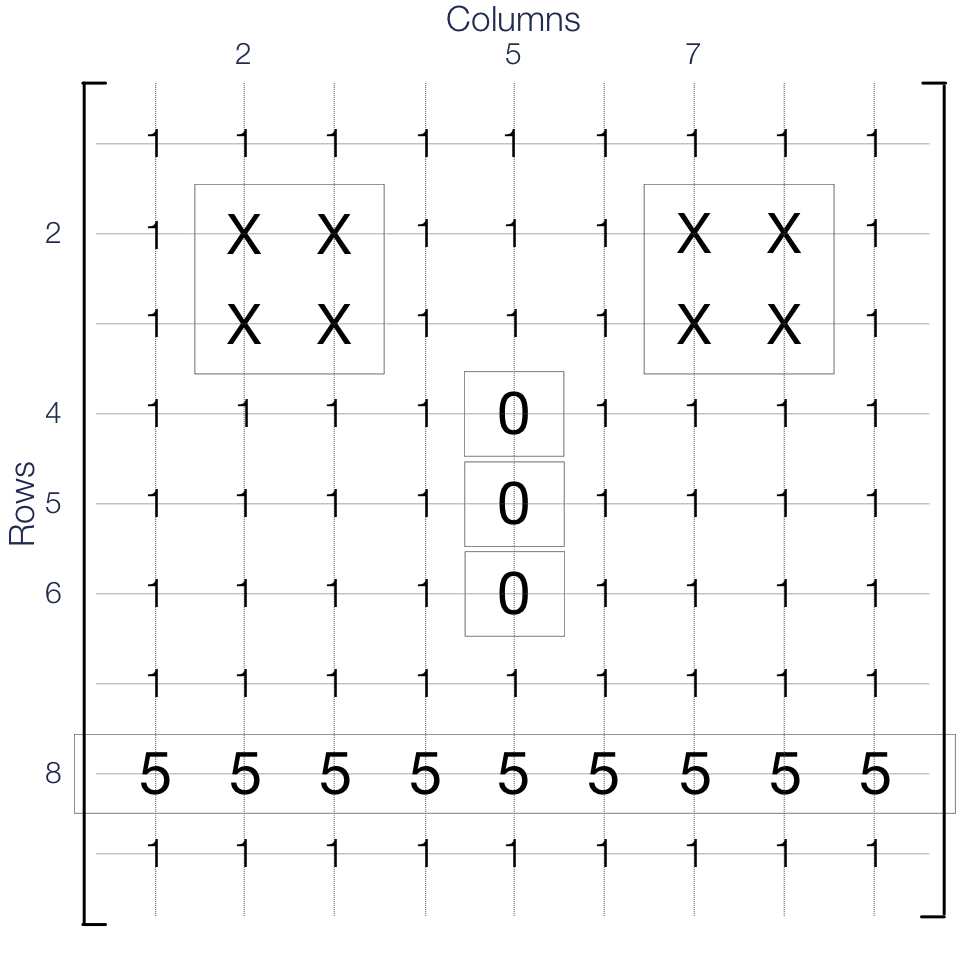
\includegraphics[width=75mm]{pics/faceMatrix.jpg}
\caption{Matrix example consisting of two blocks, three cells and one row.
They contain either numerical values or variables names. All other elements 
are defined with the attributes \xatt{diagDefault} and \xatt{offDiagDefault}, 
here both set to 1. \xelem{RowIndex} of the blocks are specified relative to 
the block start coordinates while the indexes of the cells and full matrix rows 
are absolute. The attributes \xatt{numbRows} and \xatt{numbCols} of the
matrix are required due to its sparse nature.}
\label{fig:faceMatrix}
\end{minipage}
\begin{minipage}[c]{.44\textwidth}
\lstset{language=XML}
\begin{lstlisting}
<Correlation deviationMatrixType="CovMatrix">
    <ct:VariabilityReference>
        <ct:SymbRef symbIdRef="subject"/>
    </ct:VariabilityReference>
    <Matrix symbId="faceMatrix" matrixType="Any" 
    	diagDefault="1" offDiagDefault="1">
        <!-- Left eye block -->
        <ct:MatrixBlock>
            <ct:BlockStartRow>
                <ct:Int>2</ct:Int>
            </ct:BlockStartRow>
            <ct:BlockStartColumn>
                <ct:Int>2</ct:Int>
            </ct:BlockStartColumn>
            <ct:BlockRow>
                <ct:RowIndex>
                  <ct:Int>1</ct:Int>
                </ct:RowIndex>
                <ct:SymbRef symbIdRef="X"/>
                <ct:SymbRef symbIdRef="X"/>
            </ct:BlockRow>
            <ct:BlockRow>
                <ct:RowIndex>
                   <ct:Int>2</ct:Int>
                </ct:RowIndex>
                <ct:SymbRef symbIdRef="X"/>
                <ct:SymbRef symbIdRef="X"/>
            </ct:BlockRow>
        </ct:MatrixBlock>
        <!-- Right eye block -->
        <ct:MatrixBlock>
            <ct:BlockStartRow>
                <ct:Int>2</ct:Int>
            </ct:BlockStartRow>
            <ct:BlockStartColumn>
                <ct:Int>7</ct:Int>
            </ct:BlockStartColumn>
            <!-- omitted - identical to left block -->
        </ct:MatrixBlock>
        <!-- Nose blocks -->
        <ct:MatrixCell>
            <ct:CellRow>
                <ct:Int>5</ct:Int>
            </ct:CellRow>
            <ct:CellColumn>
                <ct:Int>5</ct:Int>
            </ct:CellColumn>
            <ct:Real>0</ct:Real>
        </ct:MatrixCell>
        <!-- omitted middle cell -->
        <ct:MatrixCell>
            <ct:CellRow>
                <ct:Int>7</ct:Int>
            </ct:CellRow>
            <ct:CellColumn>
                <ct:Int>5</ct:Int>
            </ct:CellColumn>
            <ct:Real>0</ct:Real>
        </ct:MatrixCell>
        <!-- Mouth row -->
        <ct:MatrixRow default="5">
            <ct:RowIndex>
              <ct:Int>8</ct:Int>
            </ct:RowIndex>
        </ct:MatrixRow>
    </Matrix>
</Correlation>
\end{lstlisting}
\end{minipage}
\end{figure}





%\subsubsection{Example 3 -- Lower/upper triangular matrix}
%...to be finished
%

\subsubsection{Example 3 -- Block-diagonal matrix}
A typical matrix application example is the specification of the
correlation matrix of the random effects, see a screenshot for the 
Monolix GUI, Figure \ref{fig:corrMatrixMonolix}, \cite{MLXTRAN4.3.2Specification:2014}. 
This is another example of a sparse matrix with the blocks as the only non-zero 
elements of the matrix. Using attributes \xatt{diagDefault} and \xatt{offDiagDefault} 
makes the encoding an easy task leaving only the blocks to be defined explicitly. 

\begin{figure}[htb!]
\centering
  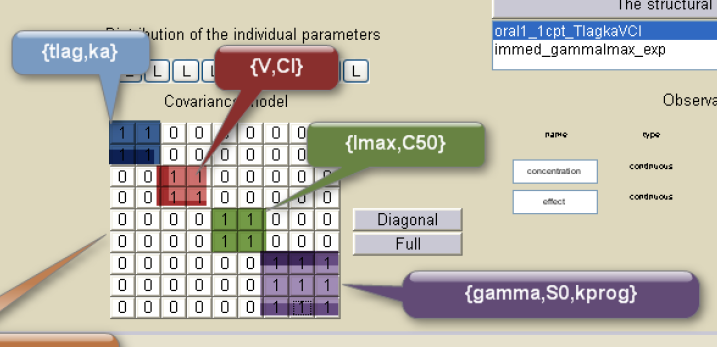
\includegraphics[width=90mm]{pics/corrMatrixMonolix}
 \caption{Correlation matrix encoded using the Monolix GUI, \cite{MLXTRAN4.3.2Specification:2014}.}
 \label{fig:corrMatrixMonolix}
\end{figure}

\lstset{language=XML}
\begin{lstlisting}
<Correlation deviationMatrixType="CorrMatrix">
    <ct:VariabilityReference>
        <ct:SymbRef symbIdRef="subject"/>
    </ct:VariabilityReference>
    <Matrix symbId="Omega" matrixType="Any" diagDefault="1" offDiagDefault="0">
        <!-- tlag, ka - block -->
        <ct:MatrixBlock>
            <ct:BlockStartRow><ct:Int>1</ct:Int></ct:BlockStartRow>
            <ct:BlockStartColumn><ct:Int>1</ct:Int></ct:BlockStartColumn>
            <ct:BlockRow>
                <ct:RowIndex><ct:Int>1</ct:Int></ct:RowIndex>
                <ct:Int>1</ct:Int><ct:Int>1</ct:Int>
            </ct:BlockRow>
            <ct:BlockRow>
                <ct:RowIndex><ct:Int>2</ct:Int></ct:RowIndex>
                <ct:Int>1</ct:Int><ct:Int>1</ct:Int>
            </ct:BlockRow>
        </ct:MatrixBlock>
        <!-- V, CL - block -->
        <ct:MatrixBlock>
            <ct:BlockStartRow><ct:Int>3</ct:Int></ct:BlockStartRow>
            <ct:BlockStartColumn><ct:Int>3</ct:Int></ct:BlockStartColumn>
            <ct:BlockRow>
                <ct:RowIndex><ct:Int>1</ct:Int></ct:RowIndex>
                <ct:Int>1</ct:Int><ct:Int>1</ct:Int>
            </ct:BlockRow>
            <ct:BlockRow>
                <ct:RowIndex><ct:Int>2</ct:Int></ct:RowIndex>
                <ct:Int>1</ct:Int><ct:Int>1</ct:Int>
            </ct:BlockRow>
        </ct:MatrixBlock>
        <!-- Imax, C50 - block -->
        <ct:MatrixBlock>
            <ct:BlockStartRow><ct:Int>5</ct:Int></ct:BlockStartRow>
            <ct:BlockStartColumn><ct:Int>5</ct:Int></ct:BlockStartColumn>
            <ct:BlockRow>
                <ct:RowIndex><ct:Int>1</ct:Int></ct:RowIndex>
                <ct:Int>1</ct:Int><ct:Int>1</ct:Int>
            </ct:BlockRow>
            <ct:BlockRow>
                <ct:RowIndex><ct:Int>2</ct:Int></ct:RowIndex>
                <ct:Int>1</ct:Int><ct:Int>1</ct:Int>
            </ct:BlockRow>
        </ct:MatrixBlock>
        <!-- gammma, S0, kprog - block -->
        <ct:MatrixBlock>
            <ct:BlockStartRow><ct:Int>7</ct:Int></ct:BlockStartRow>
            <ct:BlockStartColumn><ct:Int>7</ct:Int></ct:BlockStartColumn>
            <ct:BlockRow>
                <ct:RowIndex><ct:Int>1</ct:Int></ct:RowIndex>
                <ct:Int>1</ct:Int><ct:Int>1</ct:Int><ct:Int>1</ct:Int>
            </ct:BlockRow>
            <ct:BlockRow>
                <ct:RowIndex><ct:Int>2</ct:Int></ct:RowIndex>
                <ct:Int>1</ct:Int><ct:Int>1</ct:Int><ct:Int>1</ct:Int>
            </ct:BlockRow>
            <ct:BlockRow>
                <ct:RowIndex><ct:Int>3</ct:Int></ct:RowIndex>
                <ct:Int>1</ct:Int><ct:Int>1</ct:Int><ct:Int>1</ct:Int>
            </ct:BlockRow>
        </ct:MatrixBlock>
    </Matrix>
</Correlation>
\end{lstlisting}

%%%%%%%%%%%%%%%%%%%%%%%%%%%%%%%%%%%%%%%%%%%%%%%%%%
\subsubsection{Reading matrices}
Once a matrix is assigned, we need a mechanism for the readout of its elements. 
This is done with the \xelem{MatrixSelector} element. The following child elements 
allow flexible access to any matrix element
\begin{itemize}
\item
\xelem{SymbRef} identifies the matrix of interest (mandatory)
\item
\xelem{Cell} is used to pick one element
\item
\xelem{Block} allows to select a block of the matrix
\item
\xelem{Row} allows to select one row of a matrix
\item
\xelem{Column} allows to select one column of a matrix
\end{itemize}

\subsubsection{Example 4}
Following code shows few examples of how to access 
\begin{itemize}
\item
single element
\item
single row or
\item
\{flag,ka\} block
\end{itemize}
from the $\Omega$ matrix defined in previous example, see Figure \ref{fig:corrMatrixMonolix}.

\lstset{language=XML}
\begin{lstlisting}
            <!-- extract one element -->
            <SimpleParameter symbId="rho_tlag_ka">
                <ct:Assign>
                    <math:Equation>
                        <ct:MatrixSelector>
                            <ct:SymbRef symbIdRef="Omega"/>
                            <ct:Cell>
                                <ct:RowIndex><ct:Int>1</ct:Int></ct:RowIndex>
                                <ct:ColumnIndex><ct:Int>2</ct:Int></ct:ColumnIndex>
                            </ct:Cell>
                        </ct:MatrixSelector>
                    </math:Equation>
                </ct:Assign>
            </SimpleParameter>
            
            <!-- extract 2nd row -->
            <ct:Variable symbolType="real" symbId="SecondRow">
                <ct:Assign>
                    <math:Equation>
                        <ct:MatrixSelector>
                            <ct:SymbRef symbIdRef="Omega"/>
                            <ct:Row>
                                <ct:Int>2</ct:Int>
                            </ct:Row>
                        </ct:MatrixSelector>
                    </math:Equation>
                </ct:Assign>
            </ct:Variable>
            
            <!-- extract {tlag,ka} block -->
            <ct:Variable symbolType="real" symbId="Rho_tlag_ka">
                <ct:Assign>
                    <math:Equation>
                        <ct:MatrixSelector>
                            <ct:SymbRef symbIdRef="Omega"/>
                            <ct:Block>
                                <ct:BlockStartRow><ct:Int>1</ct:Int></ct:BlockStartRow>
                                <ct:BlockStartColumn><ct:Int>1</ct:Int></ct:BlockStartColumn>
                                <ct:RowsNumber><ct:Int>2</ct:Int></ct:RowsNumber>
                                <ct:ColumnsNumber><ct:Int>2</ct:Int></ct:ColumnsNumber>
                            </ct:Block>
                        </ct:MatrixSelector>
                    </math:Equation>
                </ct:Assign>
            </ct:Variable>
\end{lstlisting}


%\subsection{Typing rules}
%-- Subscripting has the highest precedence compared to any other arithmetic operation.


%%%%%%%%%%%%%%%%%%%%%%%%%%%%%%%%%%%%%%%%%%%%%%%%%%
%%%%%%%%%%%%%%%%%%%%%%%%%%%%%%%%%%%%%%%%%%%%%%%%%%
\section{Other changes}
\label{sec:otherChanges}
\subsection{Sum and products using indexes {\color{red} \scshape{*}}}
Sum and product symbols are frequently used in various model formulations, see for 
example section \ref{subsec:categoricalData}. Both have a very similar structure and 
consist of following elements
\begin{itemize}
\item
\xelem{SymbRef} -- to define the variable for which the sum or product is defined. 
\item
\xelem{Equation} -- sum/products can be defined for any expression {\color{red} \scshape{NEW}}.
\item
\xelem{SumIndex} or \xelem{ProductIndex} -- (optional) identifies the index.
\item
\xelem{LowLimit} and \xelem{UpLimit} -- min/max values of the index.
\item
Similarly, to vectors and matrices, indexes of sum/products can contain expressions {\color{red} \scshape{NEW}}.
\end{itemize}
Table \ref{tab:sumAndProduct} shows two basic examples of the use of sum and
product.

\begin{table}[ht!]
\setlength{\tabcolsep}{25pt}
\begin{center}
\begin{tabular}{ll}
  \hline
  \hline
 Expression &  \pml version 0.4 implementation\\
  \hline
 \multicolumn{2}{c}{Product}  \\
  \hline
$W = \prod_{i=1}^{N} V_i $
&
\lstset{language=XML}
\begin{lstlisting}
<SimpleParameter symbId="W">
    <ct:Assign>
        <math:Equation>
            <ct:Product>
                <math:Equation>
                    <ct:VectorSelector>
                        <ct:SymbRef symbIdRef="V"/>
                        <ct:Cell>
                            <ct:SymbRef symbIdRef="i"/>
                        </ct:Cell>
                    </ct:VectorSelector>
                </math:Equation>
                <ct:ProductIndex>
                    <ct:SymbRef symbIdRef="i"/>
                </ct:ProductIndex>
                <ct:LowLimit>
                    <ct:Int>1</ct:Int>
                </ct:LowLimit>
                <ct:UpLimit>
                    <ct:Int>10</ct:Int>
                </ct:UpLimit>
            </ct:Product>
        </math:Equation>
    </ct:Assign>
</SimpleParameter>
\end{lstlisting}
\\
  \hline
 \multicolumn{2}{c}{Sum}  \\
  \hline
$M = \sum_{i=1}^{N} V_i $
&
\lstset{language=XML}
\begin{lstlisting}
<SimpleParameter symbId="M">
    <ct:Assign>
        <math:Equation>
            <ct:Sum>
                <math:Equation>
                    <ct:VectorSelector>
                        <ct:SymbRef symbIdRef="V"/>
                        <ct:Cell>
                            <ct:SymbRef symbIdRef="i"/>
                        </ct:Cell>
                    </ct:VectorSelector>
                </math:Equation>
                <ct:SumIndex>
                    <ct:SymbRef symbIdRef="i"/>
                </ct:SumIndex>
                <ct:LowLimit>
                    <ct:Int>1</ct:Int>
                </ct:LowLimit>
                <ct:UpLimit>
                    <ct:SymbRef symbIdRef="N"/>
                </ct:UpLimit>
            </ct:Sum>
        </math:Equation>
    </ct:Assign>
</SimpleParameter>
\end{lstlisting}
\\
  \hline
  \end{tabular}
\vspace{-1.5em}
\caption{Implementation examples for sigma sum element, $\sum$, and product, $\prod$.}
\label{tab:sumAndProduct}
\end{center}
\end{table}


%%%%%%%%%%%%%%%%%%%%%%%%%%%%%%%%%%%%%%%%%%%%%%%%%%
\subsection{Correlation matrix update}
\label{sec:correlationMatrix}
Changes in the matrix were necessary to arrive at a consistent, generic matrix definition.
Previous format and use was determined by the correlation/covariance structure 
requirements only and was too limiting for general use. As explained in section 
\ref{sec:vectorsAndMatrices}, \xatt{matrixType} has been renamed in \xatt{deviationMatrixType}
and relocated to the \xelem{Correlation} element. The original \xatt{matrixType} 
is now populated with the names of general matrix formats. The attribute 
\xatt{deviationMatrixType} is optional and should only be used in connection with matrices.
See Figure \ref{tab:newMatrixStructure} for a comparison of the current and previous deviance 
matrix structure.

\begin{table}[ht!]
\setlength{\tabcolsep}{5pt}
\begin{center}
\begin{tabular}{ll}
  \hline
Definition in $\leq$ 0.3.1 versions 	& Definition in 0.4 version  \\
  \hline
%			\multicolumn{2}{c}{Mapping in a \xelem{CategoricalData} model}  \\  [.5ex]
  \hline
\lstset{language=XML}
\begin{lstlisting}
<Correlation>
    <ct:VariabilityReference>
        <ct:SymbRef symbIdRef="iiv"/>
    </ct:VariabilityReference>
    <Matrix matrixType="CorrMatrix">
        <ct:MatrixRow>
            <ct:Real>1</ct:Real>
            <ct:Real>2</ct:Real>
        </ct:MatrixRow>
        <ct:MatrixRow>
            <ct:Real>3</ct:Real>
            <ct:Real>4</ct:Real>
        </ct:MatrixRow>
    </Matrix>
</Correlation>
\end{lstlisting}
&
\lstset{language=XML}
\begin{lstlisting}
<Correlation deviationMatrixType="CorrMatrix">
    <ct:VariabilityReference>
        <ct:SymbRef symbIdRef="iiv"/>
    </ct:VariabilityReference>
    <Matrix matrixType="Any">
        <ct:MatrixRow>
            <ct:Real>1</ct:Real>
            <ct:Real>2</ct:Real>
        </ct:MatrixRow>
        <ct:MatrixRow>
            <ct:Real>3</ct:Real>
            <ct:Real>4</ct:Real>
        </ct:MatrixRow>
    </Matrix>
</Correlation>
\end{lstlisting}
\\
  \hline
  \end{tabular}
\vspace{-1.5em}
\caption{Changes in the matrix structure. The new attribute \xatt{deviationMatrixTyp} carries 
now values which were stored by \xatt{matrixType} in previous version, i.e. \{\xatt{CorrMatrix}, 
\xatt{CovMatrix}, \xatt{StDevCorrMatrix}, \xatt{Cholesky}\}. The attribute \xatt{matrixType} is 
now having the general values characterising a matrix, such as: \{\xatt{Any}, \xatt{LowerTriangular}, 
\xatt{UpperTriangular}, \xatt{Diagonal}, \xatt{Symmetric}\}.}
\label{tab:newMatrixStructure}
\end{center}
\end{table}


%%%%%%%%%%%%%%%%%%%%%%%%%%%%%%%%%%%%%%%%%%%%%%%%%%
\subsection{Categorical data/covariates mapping  {\color{red} \scshape{*}}}
\label{subsec:catDataCovariatesMapping}

As indicated already in section \ref{sec:catDataMapping} the mapping of category symbols 
as stored in the data set and used in the model is now done in the \xelem{ModellingSteps} 
part of PharmML. The \xelem{CategoryMapping} element is used with attributes
\begin{itemize}
\item
\xatt{dataSymbol} -- the symbol as used in the dataset, e.g. 0/1 for 'SEX' covariates
or \{1,2,3\} for categories of a categorical data model.
\item
\xatt{modelSymbol} -- the symbol as used in the model, e.g. F/M for SEX covariates
or \{cat1, cat2, cat3\} for categories of a categorical data model
\end{itemize}
see Table \ref{tab:categoryMapping} for examples.

\begin{table}[ht!]
\setlength{\tabcolsep}{1pt}
\begin{center}
\begin{tabular}{ll}
  \hline
Definition of categories  	& \xelem{CategoryMapping} in \xelem{ColumnMapping} \\
  \hline
\multicolumn{2}{c}{Mapping of discrete data categories \xelem{CategoricalData} model}  \\  [.5ex]
  \hline
\lstset{language=XML}
\begin{lstlisting}
<ObservationModel blkId="om1">

    <CategoricalData ordered="yes">
        <ListOfCategories> 
            <Category symbId="cat1"/>
            <Category symbId="cat2"/>
            <Category symbId="cat3"/>
        </ListOfCategories>
        
        <CategoryVariable symbId="Y"/>
        <!-- omitted details -->
\end{lstlisting}
&
\lstset{language=XML}
\begin{lstlisting}
<ColumnMapping>
    <ColumnRef columnIdRef="DV"/>
    <ct:SymbRef blkIdRef="om1" symbIdRef="Y"/>
    <CategoryMapping>
        <Map dataSymbol="1" modelSymbol="cat1"/>
        <Map dataSymbol="2" modelSymbol="cat2"/>
        <Map dataSymbol="3" modelSymbol="cat3"/>
    </CategoryMapping>
</ColumnMapping>


\end{lstlisting}
\\
    \hline
			\multicolumn{2}{c}{Mapping of categories of discrete covariates in \xelem{CovariateModel}}  \\  [.5ex]
  \hline
\lstset{language=XML}
\begin{lstlisting}
<CovariateModel blkId="cm1">
    <Covariate symbId="SEX">
        <Categorical>
          <Category catId="F">
              <Probability>
                  <ct:Real>.55</ct:Real>
              </Probability>
          </Category>                    
          <Category catId="M">
              <Probability>
                  <ct:Real>.45</ct:Real>
              </Probability>
          </Category>
        </Categorical>
    </Covariate>
</CovariateModel>
\end{lstlisting}
&
\lstset{language=XML}
\begin{lstlisting}
<ColumnMapping>
    <ColumnRef columnIdRef="COV"/>
    <ct:SymbRef blkIdRef="cm1" symbIdRef="SEX"/>
    <CategoryMapping>
        <Map dataSymbol="1" modelSymbol="F"/>
        <Map dataSymbol="0" modelSymbol="M"/>
    </CategoryMapping>
</ColumnMapping>
\end{lstlisting}
\\
  \hline
  \end{tabular}
\vspace{-1.5em}
\caption{Examples of category mapping for (top) discrete data categories in the categorical data model. 
(Bottom) mapping of categories of discrete covariates in \xelem{CovariateModel}.}
\label{tab:categoryMapping}
\end{center}
\end{table}


%%%%%%%%%%%%%%%%%%%%%%%%%%%%%%%%%%%%%%%%%%%%%%%%%%%
%\subsubsection{Mapping for categorical data}
%\subsubsection{Mapping for categorical covariates}

%\subsubsection{LhsTransformationType and LRhsTransformationType}
%does it matter for the users?
%- BothSideTransformation
%for 
%1. parameter model of type GaussianModel
%2. observation error of type \xelem{Standard} -  GaussianObsError 

%%%%%%%%%%%%%%%%%%%%%%%%%%%%%%%%%%%%%%%%%%%%%%%%%%
\subsection{Logarithm notation -- unified}
Previously, two symbols existed to express the natural logarithm, $\log$ and $\ln$. 
To avoid confusions, the $ln$ symbol has been removed. The following logarithm related functions
are now available
\begin{itemize}
\item
$\log$ -- the natural logarithm
\item
$\log$2 - the base-2 (binary) logarithm 
\item
$\log$10 - the base-10 (decadic) logarithm
\end{itemize}

%%%%%%%%%%%%%%%%%%%%%%%%%%%%%%%%%%%%%%%%%%%%%%%%%%
\subsection{Metadata \xatt{id}}
... is now available for every element of the schema. This allows to annotate virtually any 
element of a model.

%%%%%%%%%%%%%%%%%%%%%%%%%%%%%%%%%%%%%%%%%%%%%%%%%%
\subsection{New attribute \xatt{implementedBy} in the root element}
The new attribute \xatt{implementedBy} is helpful to keep track on the authorship of 
a PharmML encoded file. 


\lstset{language=XML}
\begin{lstlisting}
<PharmML xmlns="http://www.pharmml.org/2013/03/PharmML"
    xmlns:xsi="http://www.w3.org/2001/XMLSchema-instance"
    ...
    writtenVersion="0.4" implementedBy="JamesBond" id="i1">
    
    <ct:Name>Testing new attribute</ct:Name>
    ...
\end{lstlisting}


%%%%%%%%%%%%%%%%%%%%%%%%%%%%%%%%%%%%%%%%%%%%%%%%%%
%%%%%%%%%%%%%%%%%%%%%%%%%%%%%%%%%%%%%%%%%%%%%%%%%%
%%%%%%%%%%%%%%%%%%%%%%%%%%%%%%%%%%%%%%%%%%%%%%%%%%
\chapter{Extensions and changes in 0.4.1}
\label{ch:extensions041}

%%%%%%%%%%%%%%%%%%%%%%%%%%%%%%%%%%%%%%%%%%%%%%%%%%
%%%%%%%%%%%%%%%%%%%%%%%%%%%%%%%%%%%%%%%%%%%%%%%%%%
\section{Updated mapping of model elements and dataset}
\label{sec:updatedMapping}
This section aims to describe consistent rules for the mapping between various 
model elements such as 
\begin{itemize}
\item
administration targets
\item
continuous/discrete observations
\item
continuous/discrete covariates
\item
categories in discrete models
\item
occasions
\end{itemize}
or between selected model elements and dataset or \xelem{TrialDesign}.
Part of the mappings was available in version $\leq$ 0.4, other were missing or at least not 
explicitly described. 

Note that because of the lack \marginpar{\HandCuffLeft} of a common DDMoRe wide data format, 
the testing of the mapping implementation bas been limited in most cases to the NONMEM dataset 
although it may also work for MONOLIX data. The latter remains to be tested.

In all cases the mappings have been tested using test cases and are implemented fully in PharmML.

%Only for PK macros the mapping is implemented and tested between model and MONOLIX dataset. 

%%%%%%%%%%%%%%%%%%%%%%%%%%%%%%%%
%\subparagraph{Dataset column mapping} uses
%\begin{itemize}
%\item
%\xelem{ColumnMapping} with either
%\begin{itemize}
%\item
%\xelem{ColumnRef} and
%\item
%\xelem{SymbRef}
%\end{itemize}
%\item
%OR \xelem{ColumnMapping} with
%\begin{itemize}
%\item
%\xelem{ColumnRef} and
%\item
%\xelem{TargetMapping} with child(ren)
%\begin{itemize}
%\item
%\xelem{Map} with attributes
%\begin{itemize}
%\item
%\xatt{dataSymbol}
%\item
%\xatt{modelSymbol}
%\item
%\xatt{admNumber}
%\end{itemize}
%\end{itemize}
%\end{itemize}
%\end{itemize}
%
%%%%%%%%%%%%%%%%%%%%%%%%%%%%%%%%
%\subsubsection{\xelem{LookupTable} mapping}
%
%%%%%%%%%%%%%%%%%%%%%%%%%%%%%%%%
%\subsubsection{\xelem{TrialDesign} mapping}
%
%\xelem{TargetMapping} with child(ren)
%\begin{itemize}
%\item
%\xelem{Map} with attributes
%\begin{itemize}
%\item
%\xatt{dataSymbol}
%\item
%\xatt{modelSymbol}
%\item
%\xatt{admNumber}
%\end{itemize}
%\end{itemize}


%%%%%%%%%%%%%%%%%%%%%%%%%%%%%%%%%%%%%%%%%%%%%%%%%%
\subsection{Dosing target mapping}

%%%%%%%%%%%%%%%%%%%%%%%%%%%%%%%%%%%%%%%%%%%%%%%%%%
\subsubsection{ODE based PK model}
Note that in versions $\leq$ 0.4 the \xatt{compartmentNo} attribute 
in the \xelem{DerivativeVariable} was used for the mapping between ODE based model and the dataset. 
It has been replaced by the below described mapping for two reasons. First, to separate the model 
from the data and second in order to achieve more consistent mapping definition.

ODEs are one of the main means to encode PK models. For example, an 1-compartmental IV 
model with linear elimination reads
\begin{align}
\frac{dAc}{dt} &= - k \times Ac  \nonumber
\end{align}
which is encoded in the PharmML as the following code snippet shows
\lstset{language=XML}
\begin{lstlisting}
        <StructuralModel blkId="sm3">
            <ct:DerivativeVariable symbolType="real" symbId="Ac">
                <ct:Assign>
                    <math:Equation>
                        <math:Binop op="times">
                            <math:Uniop op="minus">
                                <ct:SymbRef blkIdRef="pm1" symbIdRef="k"/>
                            </math:Uniop>
                            <ct:SymbRef symbIdRef="Ac"/>
                        </math:Binop>
                    </math:Equation>
                </ct:Assign>
                <!-- omitted details -->
        </StructuralModel>
\end{lstlisting}
Table \ref{tab:targetMapping1} shows how the mapping between the target, $Ac$, and the 
dosing defined in either the \xelem{TrailDesing} or a NONMEM dataset is defined.
\begin{table}[ht!]
\setlength{\tabcolsep}{1pt}
\begin{center}
\begin{tabular}{ll}
  \hline
\xelem{Activity}/\xelem{TrialDesign}  	& NONMEM dataset \\
  \hline
\lstset{language=XML}
\begin{lstlisting}
<Activity oid="bolusIV"> 
  <Bolus> 
    <DoseAmount inputTarget="derivativeVariable">
      <ct:SymbRef blkIdRef="sm1" symbIdRef="Ac"/>
      <ct:Assign>
        <ct:Real>10</ct:Real>
      </ct:Assign>
   </DoseAmount>
   <DosingTimes>
      <!-- omitted details -->
   </DosingTimes>
 </Bolus>
</Activity>
\end{lstlisting}
&
\lstset{language=XML}
\begin{lstlisting}
<NONMEMdataSet oid="NMoid">

  <ColumnMapping>
    <ds:ColumnRef columnIdRef="CMT"/>
    <ds:TargetMapping blkIdRef="sm1">
      <ds:Map dataSymbol="1" modelSymbol="Ac"/>
    </ds:TargetMapping>
  </ColumnMapping>
    
  <ds:DataSet>
    <!-- omitted details -->
\end{lstlisting}
\\
  \hline
  \end{tabular}
\vspace{-1.5em}
\caption{Mapping rules for PK model encoded as an ODE for \xelem{TrialDesing} and a NONMEM dataset.}
\label{tab:targetMapping1}
\end{center}
\end{table}


%%%%%%%%%%%%%%%%%%%%%%%%%%%%%%%%%%%%%%%%%%%%%%%%%%
\subsubsection{Algebraic PK model}
Algebraic functions are used when the explicit solution for PK model is known. For example, a 
1-compartmental model with oral steady-state administration model and with linear elimination, 
based on \cite{Bonate:2011fk} p.535-537, reads
\begin{align*}
C_{SS}(t) &= \frac{D}{V}\frac{K_a}{K_a - k} \bigg(\frac{e^{-k (t-t_D)}}{1-e^{-k \tau}}-\frac{e^{-K_a (t-t_D)}}{1-e^{-K_a\tau}}\bigg) 
\end{align*}
which encoded in the PharmML reads
\lstset{language=XML}
\begin{lstlisting}
        <StructuralModel blkId="sm3">
        
            <!-- Css -->
            <ct:Variable symbolType="real" symbId="Css">
                <ct:Assign>
                    <Equation xmlns="http://www.pharmml.org/2013/03/Maths">
                        <Binop op="times">
                            <Binop op="divide">
                                <ct:SymbRef symbIdRef="D"/>
                                <ct:SymbRef blkIdRef="pm1" symbIdRef="V"/>
                            </Binop>
                            <Binop op="times">
                                <Binop op="divide">
                                    <ct:SymbRef blkIdRef="pm1" symbIdRef="Ka"/>
                                    <Binop op="minus">
                                        <ct:SymbRef blkIdRef="pm1" symbIdRef="Ka"/>
                                        <ct:SymbRef symbIdRef="k"/>
                                    </Binop>
                                </Binop>
                                <!-- omitted details -->
        </StructuralModel>
\end{lstlisting}
In this case the target is the dose parameter, D, and the following table shows how to map it.
\begin{table}[ht!]
\setlength{\tabcolsep}{1pt}
\begin{center}
\begin{tabular}{ll}
  \hline
\xelem{Activity}/\xelem{TrialDesign}  	& NONMEM dataset \\
  \hline
\lstset{language=XML}
\begin{lstlisting}
<Activity oid="bolusOR">
  <Bolus>
    <DoseAmount inputTarget="parameter"> 
      <ct:SymbRef blkIdRef="sm1" symbIdRef="D"/>
      <ct:Assign>
        <ct:Real>100</ct:Real>
      </ct:Assign>
    </DoseAmount>
    <DosingTimes>
      <!-- omitted details -->
    </DosingTimes>
  </Bolus>
</Activity>
\end{lstlisting}
&
\lstset{language=XML}
\begin{lstlisting}
<NONMEMdataSet oid="NMoid">
    
  <!-- omitted details -->
    
  <ColumnMapping>
    <ds:ColumnRef columnIdRef="AMT"/>
    <ct:SymbRef blkIdRef="sm1" symbIdRef="D"/>
  </ColumnMapping>
    
  <DataSet>
    <!-- omitted details -->
\end{lstlisting}
\\
  \hline
  \end{tabular}
\vspace{-1.5em}
\caption{Mapping rules for PK model encoded as an algebraic equation for \xelem{TrialDesing} and a NONMEM dataset.}
\label{tab:targetMapping2}
\end{center}
\end{table}

%%%%%%%%%%%%%%%%%%%%%%%%%%%%%%%%%%%%%%%%%%%%%%%%%%%
%\subsubsection{PK macros}
%PK macros are a new option extending the standard encoding ways for PK models. 
%For example, a macro for a 1-comparmental IV model with linear elimination (corresponds to ADVAN1) reads
%\lstset{language=NONMEMdataSet}
%\begin{lstlisting}
%	compartment(cmt=1, amount=Ac, volume=V)
%	iv(adm=1, cmt=1)
%	elimination(cmt=1, k)
%\end{lstlisting}
%which encoded in the proposed PharmML reads
%\lstset{language=XML}
%\begin{lstlisting}
%        <StructuralModel blkId="sm3">
%            <ct:Variable symbolType="real" symbId="Ac"/>
%            
%            <PKmacros>
%                <!-- omitted Compartment macro -->
%                <IV>
%                    <Value argument="adm">
%                        <ct:Int>1</ct:Int>
%                    </Value>
%                    <Value argument="cmt">
%                        <ct:Int>1</ct:Int>
%                    </Value>
%                </IV>
%                <!-- omitted Elimination macro -->
%            </PKmacros>
%        </StructuralModel>
%\end{lstlisting}
%The following table shows how the mapping between the target, in this case the administration 
%number identified with the attribute \xatt{adm} works for \xelem{TrailDesing} and MONOLIX dataset.
%\begin{table}[h!]
%\setlength{\tabcolsep}{1pt}
%\begin{center}
%\begin{tabular}{ll}
%  \hline
%\xelem{Activity}/\xelem{TrialDesign}  	& MONOLIX dataset \\
%  \hline
%\lstset{language=XML}
%\begin{lstlisting}
%<Activity oid="bolusIV">
%    <Bolus>
%        <DoseAmount inputTarget="admType"> 
%            <TargetMapping blkIdRef="sm3">
%                <ds:Map admNumber="1"/>
%            </TargetMapping>
%            <ct:Assign>
%                <ct:Real>100</ct:Real>
%            </ct:Assign>
%        </DoseAmount>
%        <!-- omitted details -->
%    </Bolus>
%</Activity>        
%\end{lstlisting}
%&
%\lstset{language=XML}
%\begin{lstlisting}
%<MONOLIXdataSet oid="MLXoid">
%    
%    <ColumnMapping>
%        <ds:ColumnRef columnIdRef="ADM"/>
%        <ds:TargetMapping blkIdRef="sm1">
%            <ds:Map dataSymbol="1" admNumber="1"/>
%        </ds:TargetMapping>
%    </ColumnMapping>             
%    
%    <DataSet>
%    
%    <!-- omitted details -->
%\end{lstlisting}
%\\
%  \hline
%  \end{tabular}
%\vspace{-1.5em}
%\caption{Mapping rules for macro encoded PK model for \xelem{TrialDesing} and a MONOLIX dataset.}
%\label{tab:targetMapping3}
%\end{center}
%\end{table}


%%%%%%%%%%%%%%%%%%%%%%%%%%%%%%%%%%%%%%%%%%%%%%%%%%
\subsubsection{Arbitrary model variable}
There are cases when a \emph{forcing function} in form of tabular data is provided and needs to 
be mapped to a model variable. This is the case in the so called \emph{minimal model}, used in
diabetes, of which only the relevant equation is shown
\begin{align*}
 \frac{dX(t)}{dt} & = I(t) - Ib
\end{align*}
Here, I(t) is the insulin coming from a \xelem{LookupTable}, which needs to be interpolated in 
order to convert its discrete data into continues signal required by the ODE solver. It is encoded 
in the PharmML as the following code snippet shows
\lstset{language=XML}
\begin{lstlisting}
        <StructuralModel blkId="sm1">
            
            <ct:Variable symbolType="real" symbId="I">
                <ct:Assign>
                    <ct:Interpolation>
                        <ct:Algorithm>linear</ct:Algorithm>
                        <ct:InterpIndepVar>
                            <ct:SymbRef symbIdRef="t"/>
                        </ct:InterpIndepVar>
                    </ct:Interpolation>
                </ct:Assign>
            </ct:Variable>
            
            <!-- dX(t)/dt= I(t) - Ib -->
            <ct:DerivativeVariable symbolType="real" symbId="X">
                <ct:Assign>
                <!-- omitted details -->

        </StructuralModel>
\end{lstlisting}
Table \ref{tab:targetMapping3} shows how the mapping can be defined.
\begin{table}[ht!]
\setlength{\tabcolsep}{1pt}
\begin{center}
\begin{tabular}{ll}
  \hline
\xelem{LookupTable}/\xelem{Activity}/\xelem{TrialDesign}  	& MONOLIX dataset \\
  \hline
\lstset{language=XML}
\begin{lstlisting}
<Activity oid="targetingInsulin">
  <LookupTable>
    <Target inputTarget="variable">
      <ColumnMapping>
        <ds:ColumnRef columnIdRef="INS"/>
        <ct:SymbRef blkIdRef="sm1" symbIdRef="I"/>
      </ColumnMapping>
    </Target>
    <ds:DataSet>
\end{lstlisting}
&
\lstset{language=XML}
\begin{lstlisting}
<NONMEMdataSet oid="NMoid">
    
  <ColumnMapping>
    <ds:ColumnRef columnIdRef="INS"/>
    <ct:SymbRef blkIdRef="sm1" symbIdRef="I"/>
  </ColumnMapping>
    
  <ds:DataSet>
    <!-- omitted details -->
\end{lstlisting}
\\
  \hline
  \end{tabular}
\vspace{-1.5em}
\caption{Mapping rules for arbitrary variables with input stored using \xelem{LookupTable} or a standard 
NONMEM dataset.}
\label{tab:targetMapping3}
\end{center}
\end{table}

\subparagraph{Note} Full PharmML model examples are attached to this release.


%%%%%%%%%%%%%%%%%%%%%%%%%%%%%%%%%%%%%%%%%%%%%%%%%%
\subsection{Observations mapping}
No further changes are required for the observation mapping for single observations. 
In the case when multiple DV need to be mapped the element 
\xelem{MultipleDVMapping} can be used as described in version 0.3.1 changes document \cite{Swat:2014aa}. 

%%%%%%%%%%%%%%%%%%%%%%%%%%%%%%%%%%%%%%%%%%%%%%%%%%
\subsection{Covariates mapping}
The mapping of categorical covariates has been modified already for the version 0.4 and has been
described in Section \ref{subsec:catDataCovariatesMapping} of this document.

%%%%%%%%%%%%%%%%%%%%%%%%%%%%%%%%%%%%%%%%%%%%%%%%%%
\subsection{Categorical data mapping}
The mapping of categorical covariates has been modified already for the version 0.4 and has been
described in Section \ref{subsec:catDataCovariatesMapping} of this document.

%%%%%%%%%%%%%%%%%%%%%%%%%%%%%%%%%%%%%%%%%%%%%%%%%%
\subsection{Occasions mapping}
\subsubsection{When \xelem{TrialDesign} is used}
The \xelem{TrialDesign} uses the \xelem{ObservationsEvent} element to define the occasions 
mapping as described in \cite{Pharmml_021}.

\subsubsection{When a dataset used}
In the case of datasets, the occasions are stored as covariates but need an additional 
mapping to the appropriate variability level defined in the \xelem{VariabilityLevel} encoded in 
\pml as the following snippet shows
\lstset{language=XML}
\begin{lstlisting}
        <VariabilityModel blkId="modelVar" type="parameterVariability">
            <Level symbId="indiv"/>
            <Level symbId="iov1">
                <ParentLevel>
                    <ct:SymbRef symbIdRef="indiv"/>
                </ParentLevel>
            </Level>
        </VariabilityModel>
\end{lstlisting}
Then the mapping can be defined using \xelem{ColumnMapping} element as 
described in the beginning of this section for other model elements by referring to the appropriate
symbol identifier and its block, i.e.
\lstset{language=XML}
\begin{lstlisting}
<NONMEMdataSet oid="NMoid">
    <!-- omitted details -->
    <ColumnMapping>
        <ds:ColumnRef columnIdRef="OCC"/>
        <ct:SymbRef blkIdRef="modelVar" symbIdRef="iov1"/>
    </ColumnMapping>
    
    <ds:DataSet>
        <ds:Definition>
            <ds:Column columnId="ID" columnType="id" valueType="id" columnNum="1"/>
            <ds:Column columnId="TIME" columnType="time" valueType="real" columnNum="2"/>
            <!-- omitted columns -->
            <ds:Column columnId="OCC" columnType="covariate" valueType="id" columnNum="7"/>
        </ds:Definition>
        <!-- omitted details -->
    </ds:DataSet>
</NONMEMdataSet>
\end{lstlisting}
The column OCC is mapped to \xatt{iov1} symbol, defined in the variability block \xatt{modelVar}, 
defining the inter-occasion variability level.


%%%%%%%%%%%%%%%%%%%%%%%%%%%%%%%%%%%%%%%%%%%%%%%%%%
%%%%%%%%%%%%%%%%%%%%%%%%%%%%%%%%%%%%%%%%%%%%%%%%%%
\section{\xelem{CovariateModel} and \xelem{ParameterModel} updates}
\label{sec:covariateParameterModel}

\subsubsection{Transforming and referencing covariates}
The \xelem{CovariateModel} allows to define a transformation, distribution and/or 
interpolation for a continues covariate. However, the previous \pml version didn't allow the 
distinction between the untransformed covariate and its transformed version. This had two 
disadvantages
\begin{itemize}
\item
multiple covariate models had to be defined if a covariate was to be used in parameter models 
with different transformations.
\item
accordingly multiple mappings between the various covariate models and dataset or \xelem{TrialDesign}
would be required.
\item
the covariate reference was ambiguous. For example, when using bodyweight in the dose scaling 
within the \xelem{TrialDesign} the covariate BW was applied without the transformation defined in the 
\xelem{CovariateModel}. If in the same model bodyweight was used as a covariate as well, then the 
transformed version was meant while in both cases the model would refer to the same symbol, BW. 
\end{itemize}
Let's consider, for the sake of argument, as an example the two following parameter models for 
clearance, CL, and volume, V, using both bodyweight as a covariate with and without scaling with 
respoce to the population value, respectively
\begin{align*}
 \log(CL_i) & = \log(CL_{pop}) + 0.75 \times \log \Big( \frac{BW}{70} \Big) + \eta_{CL} \Longleftrightarrow CL_i = CL_{pop}\times \Big(\frac{BW}{70} \Big)^{0.75}\times  e^{\eta_{CL}} \\
 \log(V_i) & = \log(V_{pop}) + \log(BW) + \eta_V \Longleftrightarrow V_i = V_{pop} \times BW \times e^{\eta_{V}}
\end{align*}
In PharmML $\leq$ 0.4 two covariate model blocks would be required. Instead, now only one covariate model
is necessary, but with a new \xelem{TransformedCovariate} element, as shown in the following snippet

\lstset{language=XML}
\begin{lstlisting}
        <CovariateModel blkId="cm1">
            <Covariate symbId="W">
                <Continuous>
                    <Transformation>
                        <TransformedCovariate symbId="logW70"/>
                        <math:Equation>
                            <math:Uniop op="log">
                                <math:Binop op="divide">
                                    <ct:SymbRef symbIdRef="W"/>
                                    <ct:Real>70</ct:Real>
                                </math:Binop>
                            </math:Uniop>
                        </math:Equation>
                    </Transformation>
                    <Transformation>
                        <TransformedCovariate symbId="logW"/>
                        <math:Equation>
                            <math:Uniop op="log">
                                <ct:SymbRef symbIdRef="W"/>
                            </math:Uniop>
                        </math:Equation>
                    </Transformation>
                </Continuous>
            </Covariate>
        </CovariateModel>
\end{lstlisting}
One needs to define one transformation for CL and refer to it later in the \xelem{ParameterModel}
as \xatt{logW70}, as defined within the \xelem{Transformation} tag, and another one for V, 
\xatt{logW}, see Table \ref{tab:fixedEffectsChanges}. 

Note, that if a continuous covariate is used in its unscaled form only, it is sufficient to list the covariate 
and its type as the following code snippet shows
\lstset{language=XML}
\begin{lstlisting}
        <CovariateModel blkId="cm1">
            <Covariate symbId="W">
                <Continuous/>                
            </Covariate>
        </CovariateModel>
\end{lstlisting}
using the fact that the \xelem{Transformation} element is optional. 

\begin{table}[ht!]
\setlength{\tabcolsep}{5pt}
\begin{center}
\begin{tabular}{ll}
  \hline
parameter model for CL 	& parameter model for V  \\
  \hline
  \hline
\lstset{language=XML}
\begin{lstlisting}
<?xml version="1.0" encoding="UTF-8"?>
<IndividualParameter symbId="CL">
    <GaussianModel>
        <Transformation>log</Transformation>
        <LinearCovariate>
            <PopulationParameter>
                <ct:Assign>
                    <ct:SymbRef symbIdRef="CL_pop"/>
                </ct:Assign>
            </PopulationParameter>
            <Covariate>
                <ct:SymbRef symbIdRef="logW70"/>
                <FixedEffect>
                    <ct:Real>0.75</ct:Real>
                </FixedEffect>
            </Covariate>
        </LinearCovariate>
        <RandomEffects>
            <ct:SymbRef symbIdRef="eta_CL"/>
        </RandomEffects>
    </GaussianModel>
</IndividualParameter>
\end{lstlisting}
&
\lstset{language=XML}
\begin{lstlisting}
<IndividualParameter symbId="V">
  <GaussianModel>
      <Transformation>log</Transformation>
      <LinearCovariate>
        <PopulationParameter>
          <ct:Assign>
            <ct:SymbRef symbIdRef="V_pop"/>
          </ct:Assign>
        </PopulationParameter>
        <Covariate>
          <ct:SymbRef symbIdRef="logW"/>
        </Covariate>
      </LinearCovariate>
      <RandomEffects>
        <ct:SymbRef symbIdRef="eta_V"/>
      </RandomEffects>
  </GaussianModel>
</IndividualParameter>
\end{lstlisting}
\\
  \hline
  \end{tabular}
\vspace{-1.5em}
\caption{Changes in parameter model. Fixed effect can be numerical (left) or omitted if 
not required or equal to 0 (right).}
\label{tab:fixedEffectsChanges}
\end{center}
\end{table}

\subsubsection{Redundant fixed effects}
%To allow this flexibility in encoding of models in \pml, as shown in 
%the above formulas, the \xelem{ParameterModel} had to be adjusted.
Above parameter models for CL and V in \pml version 0.4.1 as shown in Table \ref{tab:fixedEffectsChanges}
make use of two additional improvements. 

First, because the fixed effect $\beta_V$ is equal to 1, it can be simply ignored, see 
Table \ref{tab:fixedEffectsChanges} (right) where element \xelem{FixedEffect} is not present within 
\xelem{Covariate}. To allow this simplified code the \xelem{FixedEffect} element, which was 
required in previous versions, has been made optional.

\subsubsection{Numerical fixed effects}
The encoding of the parameter model for clearance in \pml 0.4.1 makes use of another 
improvement in the schema. The exponent in the covariate model for CL is fixed to 0.75. 
Before, only the assignments of symbols was allowed for fixed effects so one would have to define 
a parameter, e.g. $\beta_{CL}$, assign 0.75 to it, and use it as the fixed effect. This is now not 
necessary because \xelem{FixedEffects} can hold numerical values and not only \xelem{SymbIdRef} 
tags, see Table \ref{tab:fixedEffectsChanges} (left).
%\lstset{language=XML}
%\begin{lstlisting}
%            <IndividualParameter symbId="CL">
%                <GaussianModel>
%                    <Transformation>log</Transformation>
%                    <LinearCovariate>
%                        <PopulationParameter>
%                            <ct:Assign>
%                                <ct:SymbRef symbIdRef="CL_pop"/>
%                            </ct:Assign>
%                        </PopulationParameter>
%                        <Covariate>
%                            <ct:SymbRef symbIdRef="W70"/>
%                            <FixedEffect>
%                                <ct:Real>0.75</ct:Real>
%                            </FixedEffect>
%                        </Covariate>
%                    </LinearCovariate>
%                    <RandomEffects>
%                        <ct:SymbRef symbIdRef="eta_CL"/>
%                    </RandomEffects>
%                </GaussianModel>
%            </IndividualParameter>
%\end{lstlisting}

        
%%%%%%%%%%%%%%%%%%%%%%%%%%%%%%%%%%%%%%%%%%%%%%%%%%
%%%%%%%%%%%%%%%%%%%%%%%%%%%%%%%%%%%%%%%%%%%%%%%%%%
\section{Dose adjustment}
\label{sec:doseScaling}

Dose adjustment is a very frequent element of a PK study. Typically such adjustment means
scaling with respect to bodyweight, BW, or body surface area, BSA, or other continues covariates, 
such as creatine clearance, CLcr.

As before we have to consider different ways how such adjustment might be defined and placed
in the model. In the following we show cases for scaling which takes place either
\begin{itemize}
\item
within \xelem{ModellingSteps} when dosing information is stored in datasets or 
\item
within  \xelem{TrialDesign} using either \xelem{Bolus}/\xelem{Infusion} or \xelem{LookupTable} elements.
\end{itemize}

\subsubsection{Required extensions}
The mapping rules we presented in the section \ref{sec:updatedMapping} need to be extended 
to accommodate for dose adjustment in all these relevant cases listed above. In rare cases it is 
sufficient to map the administered amount to its target, e.g. when dose parameter D is used. 
In general however one can only map the administration compartment, CMT, but not the actual 
amount stored in the AMT column. In such cases the column mapping and the transformation 
must be linked with each other. We have introduced
\begin{itemize}
\item
new \xelem{ColumnTransformation} with the attribute \xatt{transformId} -- this is the place
when the transformation of interest is stored along with its identifier.
\item
\xelem{ColumnRef} within \xelem{ColumnMapping} gets an additional attribute 
\xatt{transformIdRef} which allows to refer to this transformation.
\end{itemize}


%%%%%%%%%%%%%%%%%%%%%%%%%%%%%%%%%%%%%%%%%%%%%%%%%%
\subsection{Scaling with dataset}
Dose scaling when a dataset is used is illustrated with two examples.

\subsubsection{Example 1 -- basic scaling example}
The scaling of a dose with the bodyweight, BW,
\begin{align*}
 & Dose_{scaled} = Dose \times BW
\end{align*}
can be encoded using the new elements, within \xelem{NONMEMdataSet} element, as shown in the 
following code snippet
\lstset{language=XML}
\begin{lstlisting}
            <!-- omitted other mappings, e.g. DV, BW, etc. -->

            <!-- step1: map CMT=1 to Ac and refer to transformation T1 -->
            <ColumnMapping>
                <ds:ColumnRef columnIdRef="CMT" transformIdRef="T1"/>
                <ds:TargetMapping blkIdRef="sm1">
                    <ds:Map dataSymbol="1" modelSymbol="Ac"/>
                </ds:TargetMapping>
            </ColumnMapping>
                        
            <!-- step2: define transformation T1 -->
            <ColumnTransformation transformId="T1">
                <math:Equation>
                    <math:Binop op="times">
                        <ds:ColumnRef columnIdRef="AMT"/>
                        <ct:SymbRef blkIdRef="cm1" symbIdRef="wgt"/>
                    </math:Binop>
                </math:Equation>
            </ColumnTransformation>
            
            <ds:DataSet>
                <ds:Definition>
                    <ds:Column columnId="ID" columnType="id" valueType="id" columnNum="1"/>
                    <ds:Column columnId="TIME" columnType="idv" valueType="real" columnNum="2"/>
                    <ds:Column columnId="DV" columnType="dv" valueType="real" columnNum="3"/>
                    <ds:Column columnId="WT" columnType="covariate" valueType="real" columnNum="4"/>
                    <ds:Column columnId="AMT" columnType="dose" valueType="real" columnNum="5"/>
                    <ds:Column columnId="CMT" columnType="cmt" valueType="int" columnNum="6"/>
                </ds:Definition>
                <!-- omitted details -->
\end{lstlisting}
First we defined the mapping of the CMT column and the target in the structural model, Ac. 
The attribute \xatt{transformIdRef} points in to the actual transformation of the administered amount.

\subsubsection{Example 2 -- complex scaling example}
We consider for a change a slightly more complex scaling law, i.e. one talking into account the creatinine 
clearance, CLcr, and dosing regimen, REGI, as a categorical covariate
\begin{align*}
 & Dose_{scaled} = Dose \times \Big(\frac{CLcr}{80}\Big)^{\theta_{clcr}} \times (1+\theta_{regi})^{REGI}
\end{align*}
which is implemented in the \xelem{NONMEMdataSet} element as the following snippet shows
\lstset{language=XML}
\begin{lstlisting}
            <!-- omitted other mappings, e.g. DV, BW, CLCR etc. -->
            <ColumnMapping>
                <ds:ColumnRef columnIdRef="CMT" transformIdRef="T1"/>
                <ds:TargetMapping blkIdRef="sm1">
                    <ds:Map dataSymbol="1" modelSymbol="Ac"/>
                </ds:TargetMapping>
            </ColumnMapping>
            
            <ColumnTransformation transformId="T1">
                <math:Equation>
                    <math:Binop op="times">
                        <ds:ColumnRef columnIdRef="AMT"/>
                        <math:Binop op="times">
                            <math:Binop op="power">
                                <math:Binop op="divide">
                                    <ct:SymbRef blkIdRef="cm1" symbIdRef="CLCR"/>
                                    <ct:Real>80</ct:Real>
                                </math:Binop>
                                <ct:SymbRef symbIdRef="theta_clcr"/>
                            </math:Binop>
                            <math:Binop op="power">
                                <math:Binop op="plus">
                                    <ct:Real>1</ct:Real>
                                    <ct:SymbRef symbIdRef="theta_regi"/>
                                </math:Binop>
                                <ct:SymbRef blkIdRef="cm1" symbIdRef="REGI"/>
                            </math:Binop>
                        </math:Binop>
                    </math:Binop>
                </math:Equation>
            </ColumnTransformation>
            
            <ds:DataSet>
                <ds:Definition>
                    <ds:Column columnId="ID" columnType="id" valueType="id" columnNum="1"/>
                    <ds:Column columnId="TIME" columnType="idv" valueType="real" columnNum="2"/>
                    <ds:Column columnId="DV" columnType="dv" valueType="real" columnNum="3"/>
                    <ds:Column columnId="CLCR" columnType="covariate" valueType="real" columnNum="4"/>
                    <ds:Column columnId="REGI" columnType="covariate" valueType="int" columnNum="5"/>
                    <ds:Column columnId="WT" columnType="covariate" valueType="int" columnNum="6"/>
                    <ds:Column columnId="AMT" columnType="dose" valueType="real" columnNum="7"/>
                    <ds:Column columnId="CMT" columnType="cmt" valueType="int" columnNum="8"/>
                </ds:Definition>
                <!-- omitted details -->
\end{lstlisting}
The \xelem{Transformation} has been introduced into the \xelem{Column} element for this
purpose.
%but the scaling when a dataset is used must be defined additionally.

\subsubsection{Example 3 -- simultaneous scaling {\color{red} \scshape{new}}}
There are occasions when one requires simultaneous scaling for two or more targets. In this 
example we show how such concurrent scaling and mapping is performed for the following design
\begin{itemize}
\item
Dosing 1: dosing to Ad is encoded in the dataset with CMT=1 and scaled by BW (transformation T1)
\item
Dosing 2: dosing to Ac is encoded in the dataset with CMT=2 and scaled by BSA (transformation T2).
\end{itemize}

\lstset{language=XML}
\begin{lstlisting}
        <!-- omitted details -->
        
        <!-- step1: map CMT=1 to Ad and refer to transformation T1 -->
        <ColumnMapping>
            <ds:ColumnRef columnIdRef="CMT" transformIdRef="T1"/>
            <ds:TargetMapping>
                <ds:Map dataSymbol="1" modelSymbol="Ad"/>
            </ds:TargetMapping>
        </ColumnMapping>
        
        <!-- step2: map CMT=2 to Ac and refer to transformation T2 -->
        <ColumnMapping>
            <ds:ColumnRef columnIdRef="CMT" transformIdRef="T2"/>
            <ds:TargetMapping>
                <ds:Map dataSymbol="2" modelSymbol="Ac"/>
            </ds:TargetMapping>
        </ColumnMapping>
        
        <!-- step3: define transformation T1 -->
        <ColumnTransformation transformId="T1">
            <math:Equation>
                <math:Binop op="times">
                    <ds:ColumnRef columnIdRef="AMT"/>
                    <ct:SymbRef blkIdRef="cm1" symbIdRef="W"/>
                </math:Binop>
            </math:Equation>
        </ColumnTransformation>
        
        <!-- step4: define transformation T2 -->
        <ColumnTransformation transformId="T2" >
            <math:Equation>
                <math:Binop op="times">
                    <ds:ColumnRef columnIdRef="AMT"/>
                    <ct:SymbRef blkIdRef="cm1" symbIdRef="BSA"/>
                </math:Binop>
            </math:Equation>
        </ColumnTransformation>
        
        <ds:DataSet>
            <ds:Definition>
                <ds:Column columnId="ID" columnType="id" valueType="id" columnNum="1"/>
                <ds:Column columnId="TIME" columnType="idv" valueType="real" columnNum="2"/>
                <ds:Column columnId="ARM" columnType="arm" valueType="id" columnNum="3"/>
                <ds:Column columnId="W" columnType="covariate" valueType="real" columnNum="4"/>
                <ds:Column columnId="BSA" columnType="covariate" valueType="real" columnNum="5"/>
                <ds:Column columnId="DOSE" columnType="dose" valueType="real" columnNum="6"/>
                <ds:Column columnId="CMT" columnType="cmt" valueType="int" columnNum="7"/>
            </ds:Definition>
            <!-- omitted details -->
        </ds:DataSet>
\end{lstlisting}


%%%%%%%%%%%%%%%%%%%%%%%%%%%%%%%%%%%%%%%%%%%%%%%%%%
\subsection{Scaling with \xelem{TrialDesign}}
The scaling when using \xelem{TrialDesign} is illustrated for two cases.

\subsubsection{Using \xelem{Bolus} or \xelem{Infusion}}
Covariate adjustment of a dose was already possible in version 0.2.1 when the definion of the 
trial design and the mapping of the associated data with a model had to be encoded in the \xelem{TrialDesign}. 
The scaling we considered in Example 1, $Dose_{scaled} = Dose \times BW$, can be encoded in 
the according \xelem{Activity} element 
\lstset{language=XML}
\begin{lstlisting}
            <Activity oid="bolusIV"> 
                <Bolus> 
                    <DoseAmount inputTarget="variable">
                        <ct:SymbRef blkIdRef="sm1" symbIdRef="Ac"/>
                        <ct:Assign>
                            <math:Equation>
                                <math:Binop op="times">
                                    <ct:Real>10</ct:Real>
                                    <ct:SymbRef blkIdRef="cm1" symbIdRef="W"/>
                                </math:Binop>
                            </math:Equation>
                        </ct:Assign>
                    </DoseAmount>
                    <!-- omitted details -->
                </Bolus>
            </Activity>            
\end{lstlisting}
This examples visualises also the advantages of the updated covariate model, see Section 
\ref{sec:covariateParameterModel}. Here we can refer the untransformed covariate bodyweight, 
W,  and the interpretation of this reference is unambiguous. 

\subsubsection{Using \xelem{LookupTable}}
This option reuses the same mapping/scaling tools as the standard datasets and will be illustrated
with mapping required in the minimal model of the infusion rate provided as \xelem{LookupTable}.
INF column is mapped to the \emph{Rglu} rate in the structural model \xatt{mmstruct} and scaled using
the bodyweight, \xatt{wgt}, as defined in the covariate model \xatt{mmcvt}.

\lstset{language=XML}
\begin{lstlisting}
<Activity oid="act4">
    <LookupTable>
        <ColumnMapping>
            <ds:ColumnRef columnIdRef="TIME"/>
            <ct:SymbRef symbIdRef="t"/>
        </ColumnMapping>
        
        <Target inputTarget="variable">
            <ColumnMapping>
                <ds:ColumnRef columnIdRef="INF" transformIdRef="T1"/>
                <ct:SymbRef blkIdRef="mmstruct" symbIdRef="Rglu"/>
            </ColumnMapping>
        </Target>
        
        <ColumnTransformation transformId="T1">
            <math:Equation>
                <math:Binop op="times">
                    <ds:ColumnRef columnIdRef="INF"/>
                    <ct:SymbRef blkIdRef="mmcvt" symbIdRef="wgt"/>
                </math:Binop>
            </math:Equation>
        </ColumnTransformation>
        
        <ds:DataSet>
            <ds:Definition>
                <ds:Column columnId="ID" columnType="id" valueType="id" columnNum="1"/>
                <ds:Column columnId="TIME" columnType="idv" valueType="real" columnNum="2"/>
                <ds:Column columnId="INF" columnType="dv" valueType="real" columnNum="3"/>
            </ds:Definition>
            <!-- omitted details -->
        </ds:DataSet>
    </LookupTable>
</Activity>
\end{lstlisting}			

%%%%%%%%%%%%%%%%%%%%%%%%%%%%%%%%%%%%%%%%%%%%%%%%%%
%%%%%%%%%%%%%%%%%%%%%%%%%%%%%%%%%%%%%%%%%%%%%%%%%%
\section{Other changes}
\label{sec:otherChanges2}


%%%%%%%%%%%%%%%%%%%%%%%%%%%%%%%%%%%%%%%%%%%%%%%%%%
\subsection{Optional \xelem{Population} element}
In the case a single subject model is considered the \xelem{Population} element
in which subjects are typically described is redundant but had been required by the \pml, 
versions $\leq$ 0.4. This has been relaxed now and the element is optional.

%%%%%%%%%%%%%%%%%%%%%%%%%%%%%%%%%%%%%%%%%%%%%%%%%%
\subsection{Additional link function}
\label{subsec:additionalLinks}
Discrete data models use so called link functions, see more details in Section \ref{subsec:mi_discreteModels}. 
Two additional are defined 
\begin{itemize}
\item
$\rm loglog$ -- the log-log function
\begin{align}
& f(\mu) = \log(-\log(\mu)) \nonumber
\end{align}
\item
$\rm comploglog$ -- the complementary log-log function
\begin{align}
& f(\mu) = \log(-\log(1-\mu)) \nonumber
\end{align}
\end{itemize}
which will make encoding of according models simpler. 


%%%%%%%%%%%%%%%%%%%%%%%%%%%%%%%%%%%%%%%%%%%%%%%%%%
\subsection{Extensions/changes in vectors and matrices}
\label{subsec:vectorsExtensions}
As indicated with red font in Sections \ref{subsec:vectorType} and \ref{subsec:matrixStructure},
elements of matrices and vectors can contain arbitrary expressions. This mean the that 
\xelem{Equation} is a new child element of \xelem{VectorElements}, \xelem{VectorCell}, 
\xelem{MatrixRow} and \xelem{MatrixCell}. Moreover, all indexes can contain expressions as well.

%%%%%%%%%%%%%%%%%%%%%%%%%%%%%%%%%%%%%%%%%%%%%%%%%%
\subsubsection{Vector elements renamed}
Two vector elements have been renamed for consistency reasons
\begin{itemize}
\item
\xelem{VectorIndex} $\longrightarrow$ \xelem{CellIndex}
\item
\xelem{SegmentIndex} $\longrightarrow$ \xelem{SegmentStartIndex}
\end{itemize}


%%%%%%%%%%%%%%%%%%%%%%%%%%%%%%%%%%%%%%%%%%%%%%%%%%
\subsection{Extensions in sums and products elements}
\label{subsec:sumProductsExtensions}

Although all of the standard and complex models, as discussed in Section \ref{subsec:mmCategoricalData}, 
were encodable in PharmML 0.4, their implementation was hampered by the missing expression 
assignments to indexes of sum/product -- this is fixed now with indexes being equipped with 
\xelem{Equation} as child element.

Additionally to the extensions marked with red in Section \ref{subsec:vectorType} and \ref{subsec:matrixStructure},
sums and products can be defined using over arbitrary expressions as well, e.g.
\begin{align}
& W = \beta_0 + \sum_{i=1}^{10} \beta_i x_i \nonumber
\end{align}
which reads as follows in PharmML
\lstset{language=XML}
\begin{lstlisting}
<SimpleParameter symbId="W">
    <ct:Assign>
        <math:Equation>
            <ct:Product>
                <math:Equation>
                    <math:Binop op="plus">
                        <ct:VectorSelector>
                            <ct:SymbRef symbIdRef="beta"/>
                            <ct:Cell>
                                <ct:Int>0</ct:Int>
                            </ct:Cell>
                        </ct:VectorSelector>
                        <math:Binop op="times">
                            <ct:VectorSelector>
                                <ct:SymbRef symbIdRef="beta"/>
                                <ct:Cell>
                                    <ct:SymbRef symbIdRef="i"/>
                                </ct:Cell>
                            </ct:VectorSelector>
                            <ct:VectorSelector>
                                <ct:SymbRef symbIdRef="x"/>
                                <ct:Cell>
                                    <ct:SymbRef symbIdRef="i"/>
                                </ct:Cell>
                            </ct:VectorSelector>
                        </math:Binop>
                    </math:Binop>
                </math:Equation>
                <ct:ProductIndex>
                    <ct:SymbRef symbIdRef="i"/>
                </ct:ProductIndex>
                <ct:LowLimit>
                    <ct:Int>1</ct:Int>
                </ct:LowLimit>
                <ct:UpLimit>
                    <ct:Int>10</ct:Int>
                </ct:UpLimit>
            </ct:Product>
        </math:Equation>
    </ct:Assign>
</SimpleParameter>
\end{lstlisting}


%%%%%%%%%%%%%%%%%%%%%%%%%%%%%%%%%%%%%%%%%%%%%%%%%%
\subsection{Discrete data -- missing element in \xelem{SimulationStep} added}
\label{subset:missingDiscrete}
The \xelem{Observation} element within \xelem{SimulationStep} is used to define the time 
points at which an observable should be simulated, as specified by the user. So far we only 
had a space holder for continues data. This has been now extended to discrete data by defining 
new element \xelem{Discrete} as the following code shows
\lstset{language=XML}
\begin{lstlisting}
        <SimulationStep oid="simStep1">
            <Observations>
                <Timepoints>
                    <ct:Sequence>
                        <ct:Begin><ct:Real>1</ct:Real></ct:Begin>
                        <ct:StepSize><ct:Real>1</ct:Real></ct:StepSize>
                        <ct:End><ct:Real>10</ct:Real></ct:End>
                    </ct:Sequence>
                </Timepoints>
                <Discrete>
                    <ct:SymbRef blkIdRef="om1" symbIdRef="y"/>
                </Discrete>
            </Observations>
        </SimulationStep>
\end{lstlisting}


%%%%%%%%%%%%%%%%%%%%%%%%%%%%%%%%%%%%%%%%%%%%%%%%%%
\subsection{Defining estimation and simulations type}
\label{subset:missingSimEst}
In \pml version $\leq$ 0.4 the description or a particular operation carried out during simulation or estimation
tasks was limited to few options, e.g. the \xatt{opType} attribute within the \xelem{Operation}
tag allowed only \xatt{estPop}, \xatt{estIndiv} and \xatt{estFIM} values. 

This restriction is now relaxed and the user can use an arbitrary string as the following code snippet shows
\lstset{language=XML}
\begin{lstlisting}
        <EstimationStep oid="estTask1">
            <TargetToolReference>
                <ct:OidRef oidRef="MLXoid"/>
            </TargetToolReference>
            <ParametersToEstimate>
                <!-- omitted details -->
            </ParametersToEstimate>
            <Operation order="1" opType="estPop"/>
            <Operation order="2" opType="estIndiv"/>
            <Operation order="3" opType="AndNowForSomethingCompletelyDifferent"/>
         </EstimationStep>
\end{lstlisting}




\bibliographystyle{plain}
\bibliography{pharmml-specification}
\end{document}





%TEMPLATES 
%% 1. Template for table with figures
%\begin{figure}[htbp]
%\centering
%\begin{tabular}{cc}
% \includegraphics[width=80mm]{pics/pic1} & 
% \includegraphics[width=80mm]{pics/pic2} \\
% \includegraphics[width=80mm]{pics/pic3} &
% \includegraphics[width=80mm]{pics/pic4}
%\end{tabular}
%\caption{about the figure}
%\label{figTable:labelText}
%\end{figure}

%\begin{table}[ht]
%\begin{center}
%\begin{tabular}{rrrrrrrrrrr}
%  \hline
% & 1 & 2 & 3 & 4 & 5 & 6 & 7 & 8 & 9 & 10 \\ 
%  \hline
%1 & 0.24 & -1.47 & -0.56 & 0.24 & 0.71 & 1.23 & 0.44 & 0.40 & 1.10 & 1.84 \\ 
%   \hline
%\end{tabular}
%\end{center}
%\end{table}
 

%\begin{figure}[htb!]
%\centering
%  \includegraphics[width=105mm]{}
% \caption{}
% \label{fig:myplot}
%\end{figure}

%PIECE-WISE
%f(z) =     \left\{ \begin{array}{rcl}
%         value1 & \mbox{for} & condition1 \\ 
%         value1 & \mbox{for} & condition1
%             \end{array}\right.


%%%%%%%%%%%%%%%%%%%%%%%%%%%%%%%%%%%%%%%%%%%%%%%%%%
% FOR LOOPS and GRUENENTHAL MODEL
%%%%%%%%%%%%%%%%%%%%%%%%%%%%%%%%%%%%%%%%%%%%%%%%%%
%%%%%%%%%%%%%%%%%%%%%%%%%%%%%%%%%%%%%%%%%%%%%%%%%%

%\subsection{For loops for categorical models}
%Loops make implementation of model simpler, especially when multiple categories have to be considered.
%Following ordered categorical model for NRS pain score, based on \cite{Wang:2014}, 
%\begin{align}
%& \text{for j = 1 to m} \nonumber \\
%  & \quad logit( P(PS <= cat_j) ) = \sum_{k=0}^{m} \beta_k + \theta_{base}(PS(t=0)-4.2) + fp(t) + f(drug) \nonumber \\ 
%& \text{end} \nonumber
%\end{align}
%has been implemented using a for-loop as the following code for the observation model shows. Note that 
%model parameters to be estimated and categories have been formulated as vectors, $\beta$ and $categoryVector$,
%respectively. Compared to the original formulation, see Figure \ref{fig:GruenenthalModel}, the subject 
%index \emph{i} of the observation variable $PS$ has been omitted.
%\lstset{language=XML}
%\begin{lstlisting}
%<ObservationModel blkId="om1">
%    <Discrete>
%        <CategoricalData>
%            <SimpleParameter symbId="m"/>
%            <SimpleParameter symbId="beta">
%                <ct:Assign>
%                    <ct:Vector>
%                        <ct:VectorElements>
%                            <ct:SymbRef blkIdRef="pm1" symbIdRef="beta_1"/>
%                            <!-- omitted beta_2 .. beta_{m-1} -->
%                            <ct:SymbRef blkIdRef="pm1" symbIdRef="beta_m"/>
%                        </ct:VectorElements>
%                    </ct:Vector>
%                </ct:Assign>
%            </SimpleParameter>
%            
%            <SimpleParameter symbId="categoryVector">
%                <ct:Assign>
%                    <ct:Vector>
%                        <ct:VectorElements>
%                            <ct:SymbRef symbIdRef="cat1"/>
%                            <!-- omitted cat_1 ... cat_{m-1} -->
%                            <ct:SymbRef symbIdRef="catm"/>
%                        </ct:VectorElements>
%                    </ct:Vector>
%                </ct:Assign>
%            </SimpleParameter>
%            
%            <ct:Variable symbolType="int" symbId="i"/>
%            <ct:Variable symbolType="int" symbId="j"/>
%            <ct:Variable symbolType="int" symbId="k"/>
%            
%            <ListOfCategories> 
%                <Category symbId="cat0"/>
%                <!-- omitted other categories -->
%                <Category symbId="catm"/>
%            </ListOfCategories>
%            
%            <CategoryVariable symbId="PS"/>
%
%        <!-- 
%        for j=1 to m
%          logit(P(PS_j<=cat_j))=\Sigma_{k=0}^{m}beta_k+theta_base*(PS_0-4.2)+fp(t)+f(drug) 
%        end 
%        -->
%            <ForLoop>
%                <ct:ProbabilityAssignment>
%                    <Probability linkFunction="logit">
%                        <math:LogicBinop op="leq">
%                            <ct:SymbRef symbIdRef="PS"/>
%                            <ct:VectorSelector>
%                                <ct:SymbRef symbIdRef="categoryVector"/>
%                                <ct:Cell>
%                                    <ct:SymbRef symbIdRef="j"/>
%                                </ct:Cell>
%                            </ct:VectorSelector>
%                        </math:LogicBinop>
%                    </Probability>
%                    <ct:Assign>
%                        <math:Equation>
%                            <math:Binop op="plus">
%                                <math:Binop op="plus">
%                                    <math:Binop op="plus">
%                                        <ct:Sum>
%                                            <math:Equation>
%                                                <ct:VectorSelector>
%                                                    <ct:SymbRef symbIdRef="beta"/>
%                                                    <ct:Cell>
%                                                        <ct:SymbRef symbIdRef="k"/>
%                                                    </ct:Cell>
%                                                </ct:VectorSelector>
%                                            </math:Equation>
%                                            <ct:SumIndex>
%                                                <ct:SymbRef symbIdRef="k"/>
%                                            </ct:SumIndex>
%                                            <ct:LowLimit>
%                                                <ct:Int>0</ct:Int>
%                                            </ct:LowLimit>
%                                            <ct:UpLimit>
%                                                <ct:SymbRef symbIdRef="m"/>
%                                            </ct:UpLimit>
%                                        </ct:Sum>
%                                        <math:Binop op="times">
%                                            <ct:SymbRef symbIdRef="theta_base"/>
%                                            <math:Binop op="minus">
%                                                <ct:VectorSelector>
%                                                    <ct:SymbRef symbIdRef="PS"/>
%                                                    <ct:Cell>
%                                                        <ct:Int>0</ct:Int>
%                                                    </ct:Cell>
%                                                </ct:VectorSelector>
%                                                <ct:Real>4.2</ct:Real>
%                                            </math:Binop>
%                                        </math:Binop>
%                                    </math:Binop>
%                                    <!-- function fp(t) -->
%                                    <math:FunctionCall>
%                                        <ct:SymbRef symbIdRef="fp"/>
%                                        <math:FunctionArgument symbId="p_max">
%                                            <ct:SymbRef blkIdRef="pm1" symbIdRef="Pmax"/>
%                                        </math:FunctionArgument>
%                                        <math:FunctionArgument symbId="k_plc">
%                                            <ct:SymbRef blkIdRef="pm1" symbIdRef="Kplc"/>
%                                        </math:FunctionArgument>
%                                        <math:FunctionArgument symbId="time">
%                                            <ct:SymbRef symbIdRef="t"/>
%                                        </math:FunctionArgument>
%                                    </math:FunctionCall>
%                                </math:Binop>
%                                <!-- function f(drug) -->
%                                <math:Binop op="divide">
%                                    <math:Binop op="times">
%                                        <ct:SymbRef blkIdRef="pm1" symbIdRef="Emax"/>
%                                        <ct:SymbRef blkIdRef="sm1" symbIdRef="C_M"/>
%                                    </math:Binop>
%                                    <math:Binop op="plus">
%                                        <ct:SymbRef blkIdRef="pm1" symbIdRef="EC50"/>
%                                        <ct:SymbRef blkIdRef="sm1" symbIdRef="C_M"/>
%                                    </math:Binop>
%                                </math:Binop>
%                            </math:Binop>
%                        </math:Equation>
%                    </ct:Assign>
%                </ct:ProbabilityAssignment>
%                <ct:LoopIndex>
%                    <ct:SymbRef symbIdRef="j"/>
%                </ct:LoopIndex>
%                <ct:StartIndex>
%                    <ct:Int>1</ct:Int>
%                </ct:StartIndex>
%                <ct:EndIndex>
%                    <ct:SymbRef symbIdRef="m"/>
%                </ct:EndIndex>
%            </ForLoop>
%        </CategoricalData>
%    </Discrete>
%</ObservationModel>
%\end{lstlisting}
%The full model is provided in the example folder as \emph{categorical\_GruenenthalModel.xml}
%
%
%\begin{figure}[htb!]
%\centering
%  \includegraphics[width=40mm,angle=-90]{pics/CategoricalWithSumModel.jpg}
% \caption{}
% \label{fig:GruenenthalModel}
%\end{figure}
